\documentclass[useAMS,usenatbib,12pt,twoside]{report}
\usepackage[margin=2.0cm]{geometry}
%\usepackage{geometry}                  
%\geometry{a4paper}
%\oddsidemargin=0.5cm %these margins aren't defined as you expect
%\evensidemargin=0.5cm
%\topmargin=0.5cm
\NeedsTeXFormat{LaTeX2e}
\usepackage{graphicx}
\usepackage{amssymb}
\usepackage{epstopdf}
\usepackage{amsmath}
\usepackage{amsthm}
\usepackage{MnSymbol}

\usepackage[round]{natbib}

\usepackage[compact]{titlesec}
%\titlespacing{\section}{0pt}{*0}{*0}
%\titlespacing{\subsection}{0pt}{*0}{*0}
\titlespacing{\subsubsection}{0pt}{*0}{*0}

\begin{document}

\newcommand{\aj}{AJ}% Astronomical Journal 
\newcommand{\araa}{ARA\&A}
          % Annual Review of Astron and Astrophys 
\newcommand{\apj}{ApJ}
          % Astrophysical Journal 
\newcommand{\apjl}{ApJ}
          % Astrophysical Journal, Letters 
\newcommand{\apjs}{ApJS}
          % Astrophysical Journal, Supplement 
\newcommand{\ao}{Appl.~Opt.}
          % Applied Optics 
\newcommand{\apss}{Ap\&SS}
          % Astrophysics and Space Science 
\newcommand{\aap}{A\&A}
          % Astronomy and Astrophysics 
\newcommand{\aapr}{A\&A~Rev.}
          % Astronomy and Astrophysics Reviews 
\newcommand{\aaps}{A\&AS}
          % Astronomy and Astrophysics, Supplement 
\newcommand{\azh}{AZh}
          % Astronomicheskii Zhurnal 
\newcommand{\baas}{BAAS}
          % Bulletin of the AAS 
\newcommand{\jrasc}{JRASC}
          % Journal of the RAS of Canada 
\newcommand{\memras}{MmRAS}
          % Memoirs of the RAS 
\newcommand{\mnras}{MNRAS}
          % Monthly Notices of the RAS 
\newcommand{\pra}{Phys.~Rev.~A}
          % Physical Review A: General Physics 
\newcommand{\prb}{Phys.~Rev.~B}
          % Physical Review B: Solid State 
\newcommand{\prc}{Phys.~Rev.~C}
          % Physical Review C 
\newcommand{\prd}{Phys.~Rev.~D}
          % Physical Review D 
\newcommand{\pre}{Phys.~Rev.~E}
          % Physical Review E 
\newcommand{\prl}{Phys.~Rev.~Lett.}
          % Physical Review Letters 
\newcommand{\pasp}{PASP}
          % Publications of the ASP 
\newcommand{\pasj}{PASJ}
          % Publications of the ASJ 
\newcommand{\qjras}{QJRAS}
          % Quarterly Journal of the RAS 
\newcommand{\skytel}{S\&T}
          % Sky and Telescope 
\newcommand{\solphys}{Sol.~Phys.}
          % Solar Physics 
\newcommand{\sovast}{Soviet~Ast.}
          % Soviet Astronomy 
\newcommand{\ssr}{Space~Sci.~Rev.} 
          % Space Science Reviews 
\newcommand{\zap}{ZAp} 
          % Zeitschrift fuer Astrophysik 
\newcommand{\nat}{Nature} 
          % Nature 
\newcommand{\iaucirc}{IAU~Circ.} 
          % IAU Cirulars 
\newcommand{\aplett}{Astrophys.~Lett.} 
          % Astrophysics Letters 
\newcommand{\apspr}{Astrophys.~Space~Phys.~Res.} 
          % Astrophysics Space Physics Research 
\newcommand{\bain}{Bull.~Astron.~Inst.~Netherlands} 
          % Bulletin Astronomical Institute of the Netherlands 
\newcommand{\fcp}{Fund.~Cosmic~Phys.} 
          % Fundamental Cosmic Physics 
\newcommand{\gca}{Geochim.~Cosmochim.~Acta} 
          % Geochimica Cosmochimica Acta 
\newcommand{\grl}{Geophys.~Res.~Lett.} 
          % Geophysics Research Letters 
\newcommand{\jcp}{J.~Chem.~Phys.} 
          % Journal of Chemical Physics 
\newcommand{\jgr}{J.~Geophys.~Res.} 
          % Journal of Geophysics Research 
\newcommand{\jqsrt}{J.~Quant.~Spec.~Radiat.~Transf.} 
          % Journal of Quantitiative Spectroscopy and Radiative Trasfer 
\newcommand{\memsai}{Mem.~Soc.~Astron.~Italiana} 
          % Mem. Societa Astronomica Italiana 
\newcommand{\nphysa}{Nucl.~Phys.~A} 
          % Nuclear Physics A 
\newcommand{\physrep}{Phys.~Rep.} 
          % Physics Reports 
\newcommand{\physscr}{Phys.~Scr} 
          % Physica Scripta 
\newcommand{\planss}{Planet.~Space~Sci.} 
          % Planetary Space Science 
\newcommand{\procspie}{Proc.~SPIE} 
          % Proceedings of the SPIE 
\newcommand{\nar}{New Astronomy Reviews} 
\newcommand{\astroussr}{Astronomical Circular U.S.S.R.} 
\newcommand{\royalsoc}{The Royal Society} 




% Misc commands
\newcommand{\tbd}{{\bf \textcolor{red}{TBD}}}
\newcommand{\sze}{Sunyaev-Zel'dovich effect }
\newcommand{\eg}{\textit{e.g.}}
\newcommand{\ie}{\textit{i.e.}}
\newcommand{\simleq}{{\raise.0ex\hbox{$\mathchar"013C$}\mkern-14mu \lower1.2ex\hbox{$\mathchar"0218$}}}
\newcommand{\simgeq}{{\raise.0ex\hbox{$\mathchar"013E$}\mkern-14mu \lower1.2ex\hbox{$\mathchar"0218$}}}
\newcommand{\newcolor}{blue}
 
 %amplitudes
%% ---- begin copy-paste ----
%% Systematic Uncertainties:
\newcommand{\mvSysTcal}{\ensuremath{0.017}}
\newcommand{\mvSysPcal}{\ensuremath{0.012}} %what is this?
\newcommand{\mvSysXtalk}{\ensuremath{0.05}}
\newcommand{\mvSysAmp}{\ensuremath{0.036}}

\newcommand{\ppSysTcal}{\ensuremath{0.017}}
\newcommand{\ppSysPcal}{\ensuremath{0.025}}
\newcommand{\ppSysXtalk}{\ensuremath{0.06}}
\newcommand{\ppSysAmp}{\ensuremath{0.038}}

%% Measured Amplitudes:
\newcommand{\mvAmp}{\ensuremath{0.94}}
\newcommand{\mvAmpStat}{\ensuremath{0.05}}
\newcommand{\mvAmpSys}{\ensuremath{0.04}} %0.041
\newcommand{\mvAmpUnlStat}{\ensuremath{0.02}}

\newcommand{\ppAmp}{\ensuremath{0.99}}
\newcommand{\ppAmpStat}{\ensuremath{0.09}}
\newcommand{\ppAmpSys}{\ensuremath{0.05}} %0.048
\newcommand{\ppAmpUnlStat}{\ensuremath{0.05}}

%% Measured Significances:
\newcommand{\mvSig}{\ensuremath{17.1 \sigma}} % 0.94/0.05
\newcommand{\mvSigUnl}{\ensuremath{41 \sigma}} % 0.94/0.02
\newcommand{\mvPercent}{\ensuremath{ 6 \%}} % 0.05/0.94
\newcommand{\ppSig}{\ensuremath{11.1 \sigma}} % 0.99/0.09
\newcommand{\ppSigUnl}{\ensuremath{19.8 \sigma}} % 0.99/0.05
\newcommand{\ppPercent}{\ensuremath{ 9 \%}} % 0.09/0.99

%% Total Amplitude Errors:
\newcommand{\mvDampTot}{\ensuremath{0.10}} % sqrt(0.0830**2 + 0.0546**2)
\newcommand{\ppDampTot}{\ensuremath{0.14}} % sqrt(0.1134**2 + 0.0884**2)

%% Clpp significances:
\newcommand{\mvTotPercent}{\ensuremath{11 \%}} % 0.10/0.94
\newcommand{\ppTotPercent}{\ensuremath{15 \%}} % 0.14/0.99
\newcommand{\mvTotSig}{\ensuremath{9.4 \sigma}} % 0.94/0.10
\newcommand{\ppTotSig}{\ensuremath{6.9 \sigma}} % 0.99/0.14

%% Spectrum PTE's:
\newcommand{\mvPTE}{\ensuremath{0.92}}
\newcommand{\ppPTE}{\ensuremath{0.71}}

\newcommand{\mvLCDMSig}{\ensuremath{0.65 \sigma}}
\newcommand{\ppLCDMSig}{\ensuremath{0.10 \sigma}}


%% ---- end copy-paste ----

\newcommand{\nbin}{\ensuremath{10}}


\newcommand{\nhat}{\ensuremath{\mathbf{\hat{n}}}}
\newcommand{\aalpha}{\ensuremath{\vec{\bf \alpha}}}
 \newcommand{\sigT}{\mbox{$\sigma_{\mbox{\tiny T}}$}}
 \newcommand{\Tcmb}{\mbox{$T_{\mbox{\tiny CMB}}$}}
 \newcommand{\neff}{\ensuremath{N_\mathrm{eff}}\xspace}
 \newcommand{\yhe}{\ensuremath{Y_p}}
 \newcommand{\As}{\ensuremath{A_s}}
 \newcommand{\deltaR}{\ensuremath{\Delta_R^2}}
 \newcommand{\nrun}{\ensuremath{dn_s/d\ln k}\xspace}
 \newcommand{\alens}{\ensuremath{A_{L}}}
 \newcommand{\ns}{\ensuremath{n_{s}}}
 \newcommand{\ho}{\ensuremath{H_{0}}\xspace}
 \newcommand{\muksq}{\ensuremath{\mu{\rm K}^2}}
 \newcommand{\sumnu}{\ensuremath{\Sigma m_{\nu}}}
 \def\microKsq{\mu{\mbox{K}}^2}
 \def\muKarcmin{\mu K . {\rm arcmin}}
 \def\mb{\mathbf}
 \newcommand{\sqdeg}{\ensuremath{\rm deg^2~}}
 \newcommand{\kappam}{\ensuremath{\kappa~}}
 \def\deg{^\circ}

% experiments
 \newcommand{\wmap}{\textit{WMAP}}
 \newcommand{\wseven}{\textit{WMAP}7}
 \newcommand{\sptpol}{SPTpol~}
 \newcommand{\planck}{\textit{Planck}}
 \newcommand{\polarbear}{POLARBEAR}
 \newcommand{\bicep}{BICEP2}
 \newcommand{\keck}{KECK Array}
 \hyphenation{BICEP}
 \hyphenation{POLAR-BEAR}

\def\microKsq{\mu{\mbox{K}}^2}
 \def\muKarcmin{$\mu{\mbox{K}}$-arcmin}

 \def\mb{\mathbf}     % ``math-bold''
 \def\mbL{\mathbf{L}} % math-bold L
 \def\mbell{\pmb{\ell}} % math-bold ell
 \def\tbd{\textcolor{red}{TBD}}

 \def\cl{$C_{\ell}$\xspace}
 \def\clnospace{\ensuremath{C_{\ell}}}
 \def\dl{$D_{\ell}$}

 % power spectrum expressions
 \def\clpp{\ensuremath{C^{\phi \phi}_L}}
 \def\clppHat{\ensuremath{C^{\hat{\phi} \hat{\phi}}_L}}
 \def\clppHatUVXYL{\ensuremath{C^{\hat{\phi}^{UV} \hat{\phi}^{XY}}_{\mbL}}}
 \def\cmbLppHat{\ensuremath{C^{\hat{\phi} \hat{\phi}}_{\mbL}}}
 \def\hatcmbLpp{\ensuremath{\hat{C}^{\phi \phi}_{\mbL}}}
 \def\hatclppUVXYb{\ensuremath{\hat{C}^{\phi^{UV} \phi^{XY}}_b}}
 \def\hatclppUVXYL{\ensuremath{\hat{C}^{\phi^{UV} \phi^{XY}}_{\mbL}}}

 \def\hatclkkUVXYb{\ensuremath{\hat{C}^{\kappa^{UV} \kappa^{XY}}_b}}
 \def\hatclkkUVXYL{\ensuremath{\hat{C}^{\kappa^{UV} \kappa^{XY}}_{\mbL}}}

 % bias terms
 \def\dclNzero{\ensuremath{\left. \Delta C_{\mbL}^{\phi \phi}\right|_{\rm N0}}}
 \def\dclRDNzero{\ensuremath{\left. \Delta C_{\mbL}^{\phi \phi}\right|_{\rm RDN0}}}
 \def\dclNone{\ensuremath{\left. \Delta C_{\mbL}^{\phi \phi}\right|_{\rm N1}}}
 \def\dclMC{\ensuremath{\left. \Delta C_{\mbL}^{\phi \phi}\right|_{\rm MC}}}
 
 \def\mv{MV}
 \def\pp{POL}

\def\be{\begin{equation}}
\def\ee{\end{equation}}
\def\ba{\begin{eqnarray}}
\def\ea{\end{eqnarray}}
\def\nn{\nonumber}
%%%%%%%%%%%%%%%%%%%%%%%%%%%%%%%%%%%%%%%%%%%%%%%%%%%%%%%%%%%%%%%%%%
% This is in my opinion a way better way of writing any large work in latex. You can work on each chapter individually without getting lost this way. I also found seeing all the chapter headings with to-do's under them helped me keep a good overview of where I was up to. I haven't included all my chapters, but I've left them in below, commented out, to give you an idea of how it looks.
%%%%%%%%%%%%%%%%%%%%%%%%%%%%%%%%%%%%%%%%%%%%%%%%%%%%%%%%%%%%%%%%%%

\pagestyle{empty}
  
\begin{center}
\vspace{2.0cm}
\Huge
\bfseries
\text{\bfseries{Searching for the Missing Baryon Fraction}}\\
\text{\bfseries{with \sptpol and the Dark Energy Survey}}\\
\mdseries
\vspace{2.0cm}
\Large{Mitchell de Zylva}\\
\vspace{1.0cm} % stands for vertical space. Fiddle with as needed
\large{
Supervised by\\
Dr Chrisitan Reichardt\\}
\vspace{4.0cm}
\Large{School of Physics}\\
\large{Faculty of Science}\\
\large{University of Melbourne\\}
\vspace{0.5cm}
%\text{[logo goes here]\\} %comment out this line and uncomment the next when you have a nice uni logo...

\includegraphics[width = 0.25\textwidth]{logo.pdf}\\

\vspace{2.0cm}
%\Large{25 October, 2010\\}
\Large{\today \\}
\vspace{0.5cm}
\normalsize
Submitted in fulfillment of the requirements of the degree of\\
Master of Science (Physics)
\end{center}
  


\bfseries{Statement of contribution:}\mdseries\\
\vspace{1.0cm}

This is to certify that:\\

\begin{itemize}

\item This thesis entitled ``Studying weakly lensed galaxies
with velocity maps'' comprises only my original work except where indicated otherwise.

\item Due acknowledgement has been made in the text to all other material used.

\item The thesis is no longer than 50 pages in length, inclusive of tables, figures, bibliographies and
appendices.

\end{itemize}

\vspace{4.0cm}


\scriptsize{..........................................................}\normalsize\\
\newline
\vspace{3.0cm}
\indent Mitchell de Zylva\\
      					 
\vspace{2.0cm}

\bfseries{Acknowledgements:}\mdseries\\

You put all the people you want to thanks here :)\\

You need a statement of contribution, which you will sign before you submit. 
	\begin{abstract}

Abstract goes here..

\end{abstract} % This is a separate file. See example
\pagestyle{plain}
 	\setcounter{page}{4} %the cover page doesn't count as a page
 	\tableofcontents
% 	\listoffigures  % you probably don't need this	
 	
	\chapter{Introduction}
	%  - Introduction 
			%- 	CMB 
			%- 	Cosmological Parameters
\section{Modern Cosmology, and the Cosmic Microwave Background}
Modern cosmology has been experiencing a golden age since the 1990s. Access to larger and larger datasets has allowed astronomers to develop increasingly more detailed models of the universe. These models rely on several fundamental assumptions stemming from observation, the chief of which is the Big Bang Model. 
\par In 1929, Edwin Hubble confirmed a relation earlier found by Georges Lemaître, between  distances to galaxies and their recessional velocities: galaxies appear to be moving faster away from us, the further away they are \citep{1929PNAS...15..168H}. These observations gave rise to the Hubble Law,
\begin{equation}
	v  \varpropto d
	\label{eq:HubbleLaw}
\end{equation}
where $v$ is the velocity of a galaxy in question, and $d$ is its distance from us. 
\par To the best of our knowledge, there is nothing that suggests that our position in the universe is special or unique, a concept known as the Copernican Principle \citep{peacock_peacock_1998}. This leads to the logical extension that if every point in the universe is moving away from every other point, the universe must be expanding. If we reverse the flow of time, the universe must have been an incredibly hot, dense environment at some point in the past, a singularity known as the \emph{Big Bang}.
\par This singularity then expanded outwards, bringing into existence the early universe. Small fluctuations present in quantum fields, resulting from Heisenberg's Uncertainty Principle, created small inhomogeneities which seeded the universe with elementary quantum objects, such as quarks, gluons, photons, and dark matter. These particles swirled in a primordial fluid, mixing together, until eventually the universe cooled to a point that all the elements of the mixture stopped interacting with (i.e. de-couple from) each other. 
\par This early exponential expansion allowed the universe to mix, and so achieve a very high level of isotropy. Observationally, there appears to be no favoured direction in the universe, since distributions of distant galaxies and other extragalactic sources seem to be even across the sky. Perhaps the most spectacular example of this isotropy is the presence of the \emph{Cosmic Microwave Background} (CMB).
\par Discovered in 1964 \citep{Penzias:65} as a source of noise in another microwave experiment, over the next 30 years, it was noticed that there was isotropic black-body radiation everywhere in the universe, at a temperature of $T \approx \SI{2.7}{\kelvin}$. This radiation is most intense in the microwave section of the electromagnetic spectrum, it was named the cosmic microwave background.
\begin{figure}[ht]
	\centering
	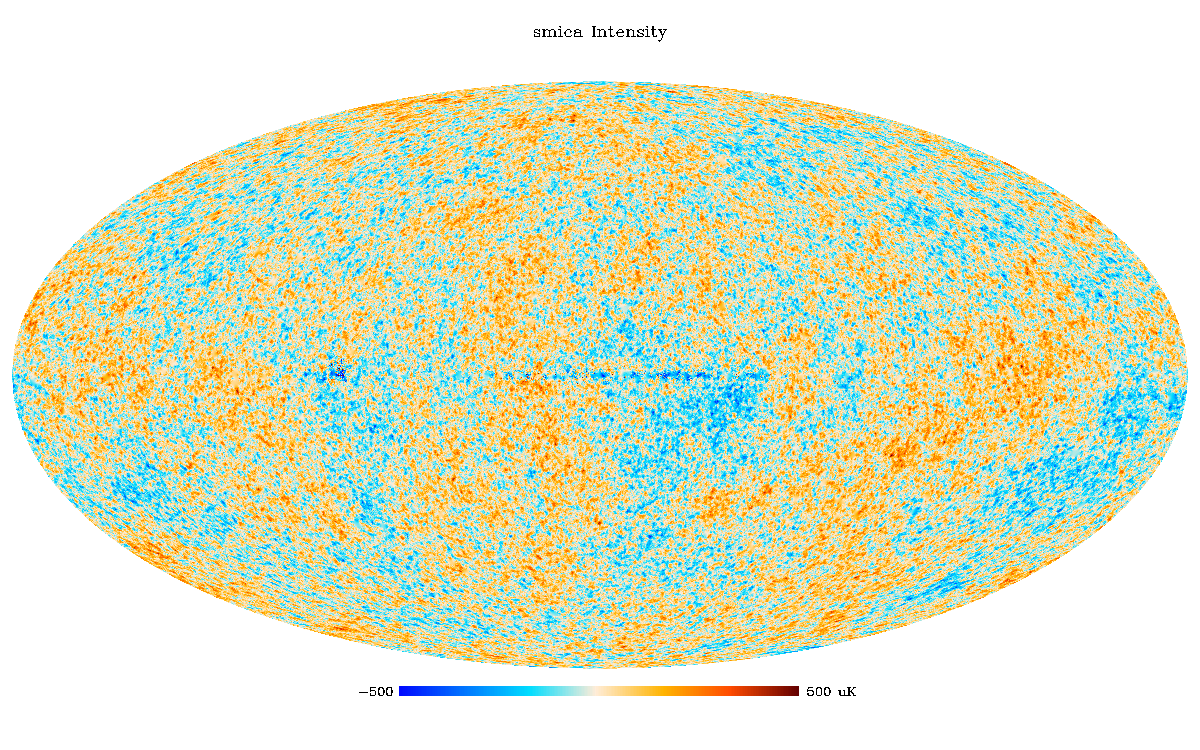
\includegraphics[scale=0.25]{/home/mitchell/Documents/masters/masters/thesis/Images/CMB_smica_tsig.png}
	\label{CMB Map}
	\caption{\emph{Planck} Satellite Full Sky CMB Map, extracted using the SMICA method \citep{2018arXiv180706205P}. This  map was produced by linearly combining the full spectrum of frequencies observed by the \emph{Planck} satellite from $\SI{30}{\giga\hertz}$ to $\SI{857}{\giga\hertz}$ in frequency space. Each map is first converted to its power spectrum, and then weighted at various multipoles, in order to account for contamination which appears at characteristic scales in different frequencies.}
\end{figure}

The CMB is a near-perfectly uniform field of background radiation which permeates the universe. Intially believed to be featureless, today the CMB is known to have very specific inhomogenaities, shown in \ref{CMB Map}. The uniformity of the CMB is the closest measurement we have to a perfect black-body, but with variations of approximately one part in 100,000, and an RMS of $\SI{18}{\micro\kelvin}$ \citep{2004mmu..symp..291W}. 

Theory holds that a very short time after the Big Bang ($\sim 10^{-37}$ seconds), the universe underwent an exponential growth period now termed \textit{inflation}. This phase is necessary to ensure that the universe is isotropic, flat, and gaussian, whilst also still taking into account the fact that opposite sides of the observable universe appear to be too far apart to ever have been causally connected. During this period, the universe was smoothed out, only leaving behind very small irregularities. These irregularities are what eventually gives rise to the large scale structure of the universe, what eventually would become the \emph{Cosmic Web}. 

As the universe adiabatically cooled, there was a considerable period of time, until approximately 380,000 years after the Big Bang, where photons were coupled to the other components of the universe, such as baryonic matter and dark matter. This period is what allowed for the quark-gluon plasma to mix appropriately, and develop waves in the fluid, ultimately resulting in the characterstic pattern in the CMB. This pattern is highly dependant on statistical parameters, and so the characterisitic angular size of the pattern of the CMB is incredibly sensitive to the relative proportions of the universe's matter-energy density. These charactersitic inhomogeneities can be decomposed into an angular power spectrum, which exibits a shape highly dependant on universal parameters. 

\begin{figure}[h!]
\centering
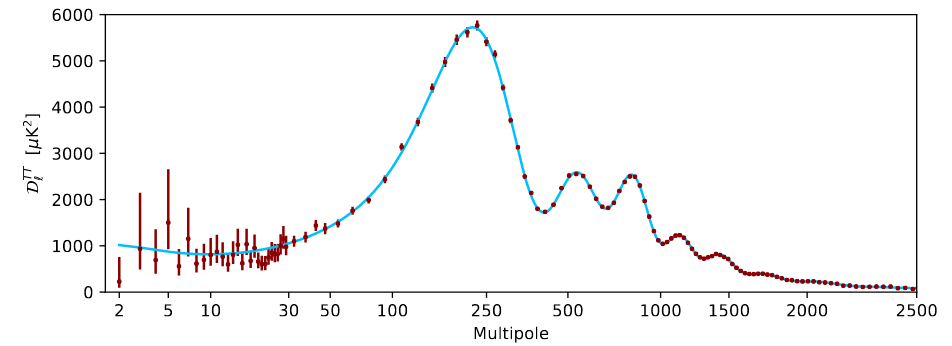
\includegraphics[scale=0.4]{/home/mitchell/Documents/masters/masters/thesis/Ver_2/figures/planck_2018.png}
\caption{\emph{Planck} 2018 Angular Power Spectrum \citep{2018arXiv180706209P}. The location, and relative heights of the first three peaks are sensitive to the overall energy density of the universe, as well as the relative amounts of baryonic matter and dark matter.}
\label{fig:power_spec}
\end{figure}

Shown in Figure \ref{fig:power_spec}, this angular power spectrum is very sensitive to cosmological paramters. Since the discovery of its anisotropy by \emph{Cosmic Background Explorer} (COBE) \citep{1992PhT....45f..17L}, and then its later refinement by \textit{Wilkinson Microwave Anisotropy Probe} (WMAP) \citep{2007ApJS..170..377S}, the power spectrum has been the gold standard by which astronomers measure cosmological parameters. The precision to which we know the CMB also makes it very good as constraining these parameters, leading many cosmologists to hold it as one of the most accurate measurements ever made in physics.  

\section{Cosmological Parameters}
The current accepted model, the $\Lambda$CDM model, contains six independant paramters which describe the evolution and behaviour of the universe: the physical baryon density $\Omega_b h^2$, the physical dark matter density $\Omega_c h^2$, the age of the universe $t_0$, the scalar spectral index $n_s$, the acoustic scale $100 \theta_\star$, and the reionisation optical depth $\tau$, the values of which are reported in Table \ref{table:params}. These primary parameters give rise to other parameters, such as the Hubble constant $H_0$ and its unitless form, known as the reduced Hubble constant $h$. It serves as a measure of the current rate of expansion of the universe, and carries units of $ \SI{}{\kilo\meter\per\second\per\mega\parsec}$. The Hubble constant is usually quoted for a number of reasons. Firstly, it contains both the age, and the size, of the universe within it, and secondly, it was one of the first cosmological parameters to be determined, back when Hubble was making his initial measurements, so it has some historical value. Because it is so ubiquitous, astronomers use different forms depending on what they are analysing, which becomes important for making direct comparisons between different measurements. When using the unitless form, if it lacks a subscript, it refers to the definition $h = H_0/\SI{100}{\kilo\meter\per\second\per\mega\parsec}$. Alternatively, if it carries one, it refers to replacing the number in the denominator with the number in the subscript, e.g. $h_{70} = H_0/\SI{70}{\kilo\meter\per\second\per\mega\parsec}$.

Currently, the highest precision measures of these features from the CMB come from the  \cite{2018arXiv180706209P} paper, which details that baryonic matter only comprises $\approx 5 \% $ of the universe's energy density. 

\par In principle, this component of the universe should be directly measurable. At just three minutes after the Big Bang, deuterium can be used as a tracer for this abundance \citep{2007ARNPS..57..463S}, and at a redshift $z \geqslant 2$, the baryon fraction can be found in the absorption lines of quasars passing through the diffuse, photo-ionised intergalactic medium, known as the Lyman-$\alpha$ forest \citep{1997ApJ...490..564W}. 

\par The baryon content has been confirmed very well at high redshift by the Planck collaboration, and the agreement between the CMB, and other independant high redshift measurements, such as baryon acousitc oscillations, and gravitational lensing reconstructions .  

\par However as the universe evolved, this gas became sparser, both as space expanded, and as it became more ionised by processes in the universe. This makes searching for the entirety of the baryon fraction at low redshift difficult, since high density objects are usually more easily detected. When this fraction is calculated for the local universe directly from observations, it shows only one tenth of the baryonic content shown in high redshift measurements is contained in galactic structures \citep{1992MNRAS.258P..14P}. This is troubling, because tensions in cosmological parameters between their high and low redshift measurments forces us to ask questions about the validity of cosmological models at all times.

\begin{table}[h!]
\centering
\begin{tabular}{||c c c||} 
 \hline
 Parameter & Value & Error \\
 \hline\hline
 $\Omega_c h^2$ & $0.120$ & $\pm 0.001$ \\
 \hline
 $\Omega_b h^2$ & $0.0224$ & $\pm 0.0001$ \\
 \hline
  $n_s$ & $0.965$ & $\pm 0.004$ \\
 \hline
  $\tau$  & $0.054$ & $\pm 0.007$ \\
 \hline
  $100 \Theta_\star$ & $1.0411$ & $\pm 0.0003$ \\
 \hline
 $H_0$ (km s$^{-1}$ Mpc$^{-1}$) & $67.4$ & $\pm 0.5$ \\
 \hline

\end{tabular}
\caption{Latest Reported Values for Cosmological Parameters from the \emph{Planck} Satellite \citep{2018arXiv180706209P}.}
\label{table:params}
\end{table}




 	
 	% Motivation
 	% Basic Grav lensing 
	%etc 
	 
	%\include{Ellipse_fitting}
	
	% Making galaxies or importing them 
	% Shearing galaxies
	% Determining the shear
	% Velocity curve and inclination angle
	% Fitting ellipses
	
	
\chapter{Results}

From the process outlined above, 787,058 galaxy pairs were constructed with a mean angular separation of $\sim 27.6 $ arcmins, and a mean comoving separation of $11.9 h^{-1}$ Mpc. 

\begin{figure}[H]
\centering
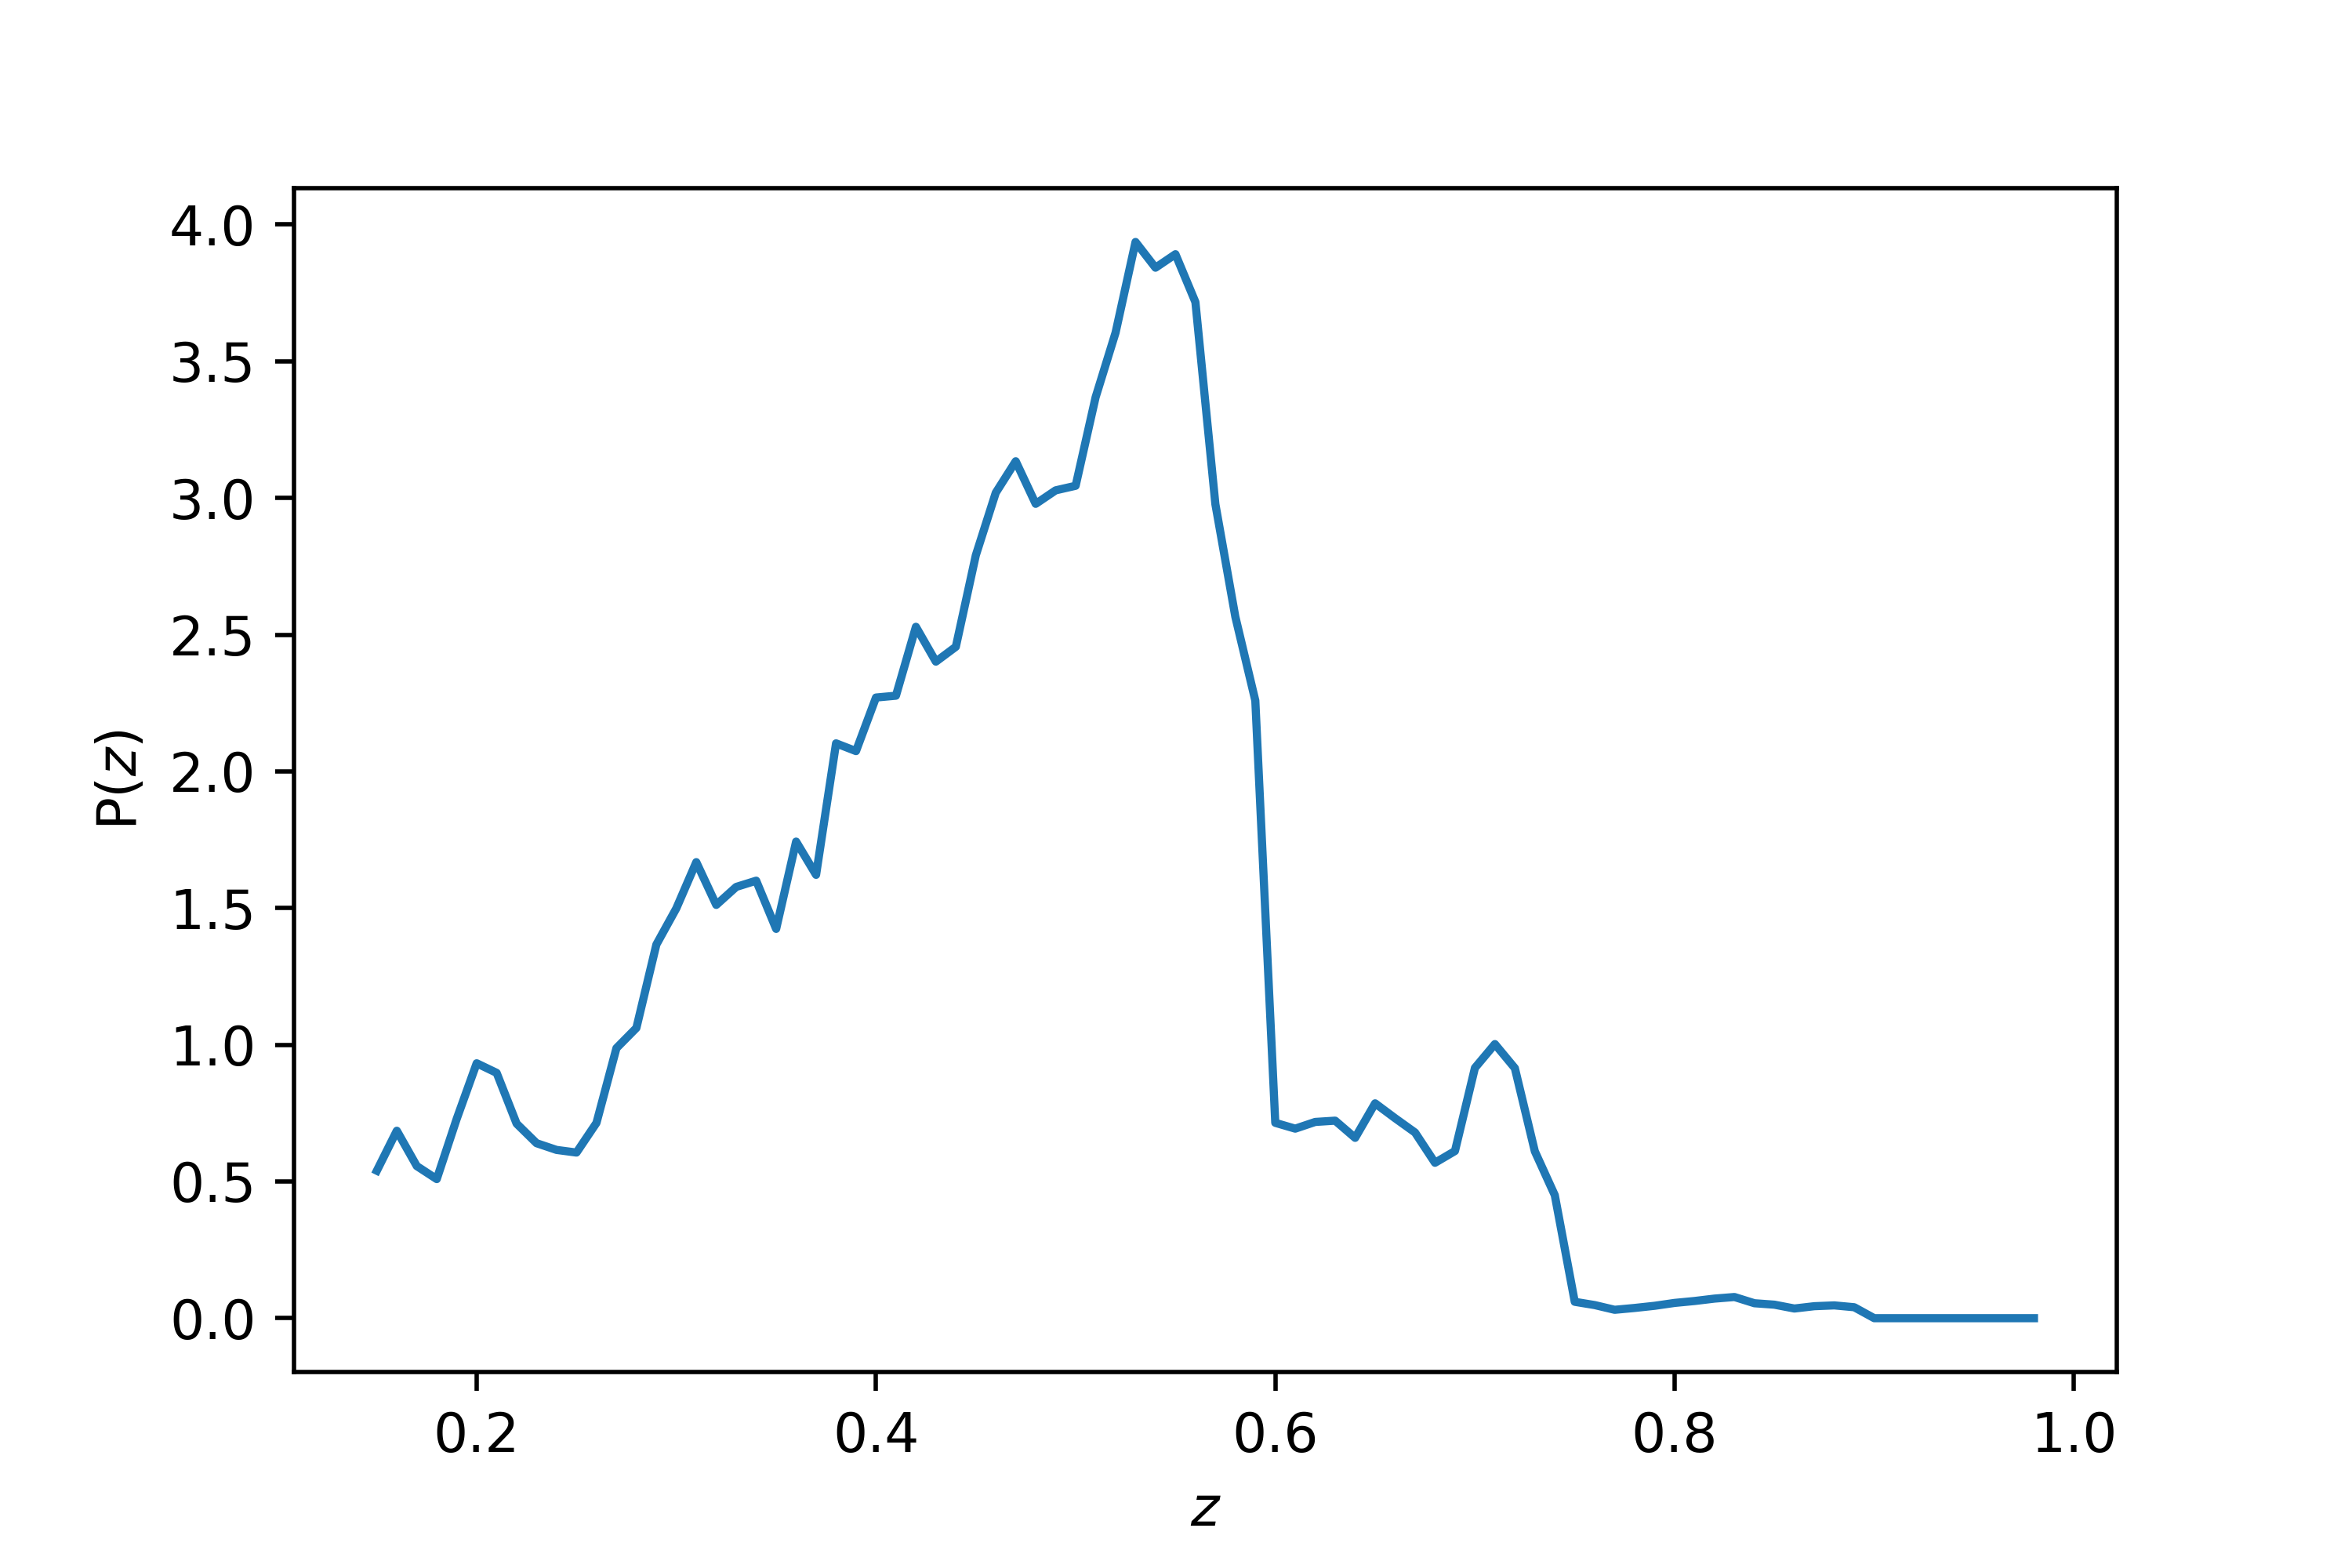
\includegraphics[width=0.6\textwidth , keepaspectratio]{/home/mitchell/Documents/masters/masters/thesis/Ver_2/figures/Redshift_Distribution.png}
\caption{Redshift Distributions of Physical Pairs. The pairs range from redshifts $z\approx0.15$ to $z\approx0.90$, with a mean redshift of $z\approx0.50$.}
\label{fig:physical:redshifts}
\end{figure}

Figure \ref{fig:physical:redshifts} shows the overall PDF of galaxy pairs as a function of redshift. It shows that the mean redshift for the pairs is $z=0.468$, with a minimum redshift of $z= 0.15$, and a maximum redshift of $z= 0.90$. There is a rather drastic drop in the galaxy population after redshift $z \sim 0.58$. This is due to there being fewer galaxies in the higher redshift bins in the DES Year 1 Catalogue. Figures \ref{fig:physical:lineofsight} and \ref{fig:physical:transverse} show the line-of-sight and transverse separation PDFs of the pairs.

\begin{figure}[H]
\centering
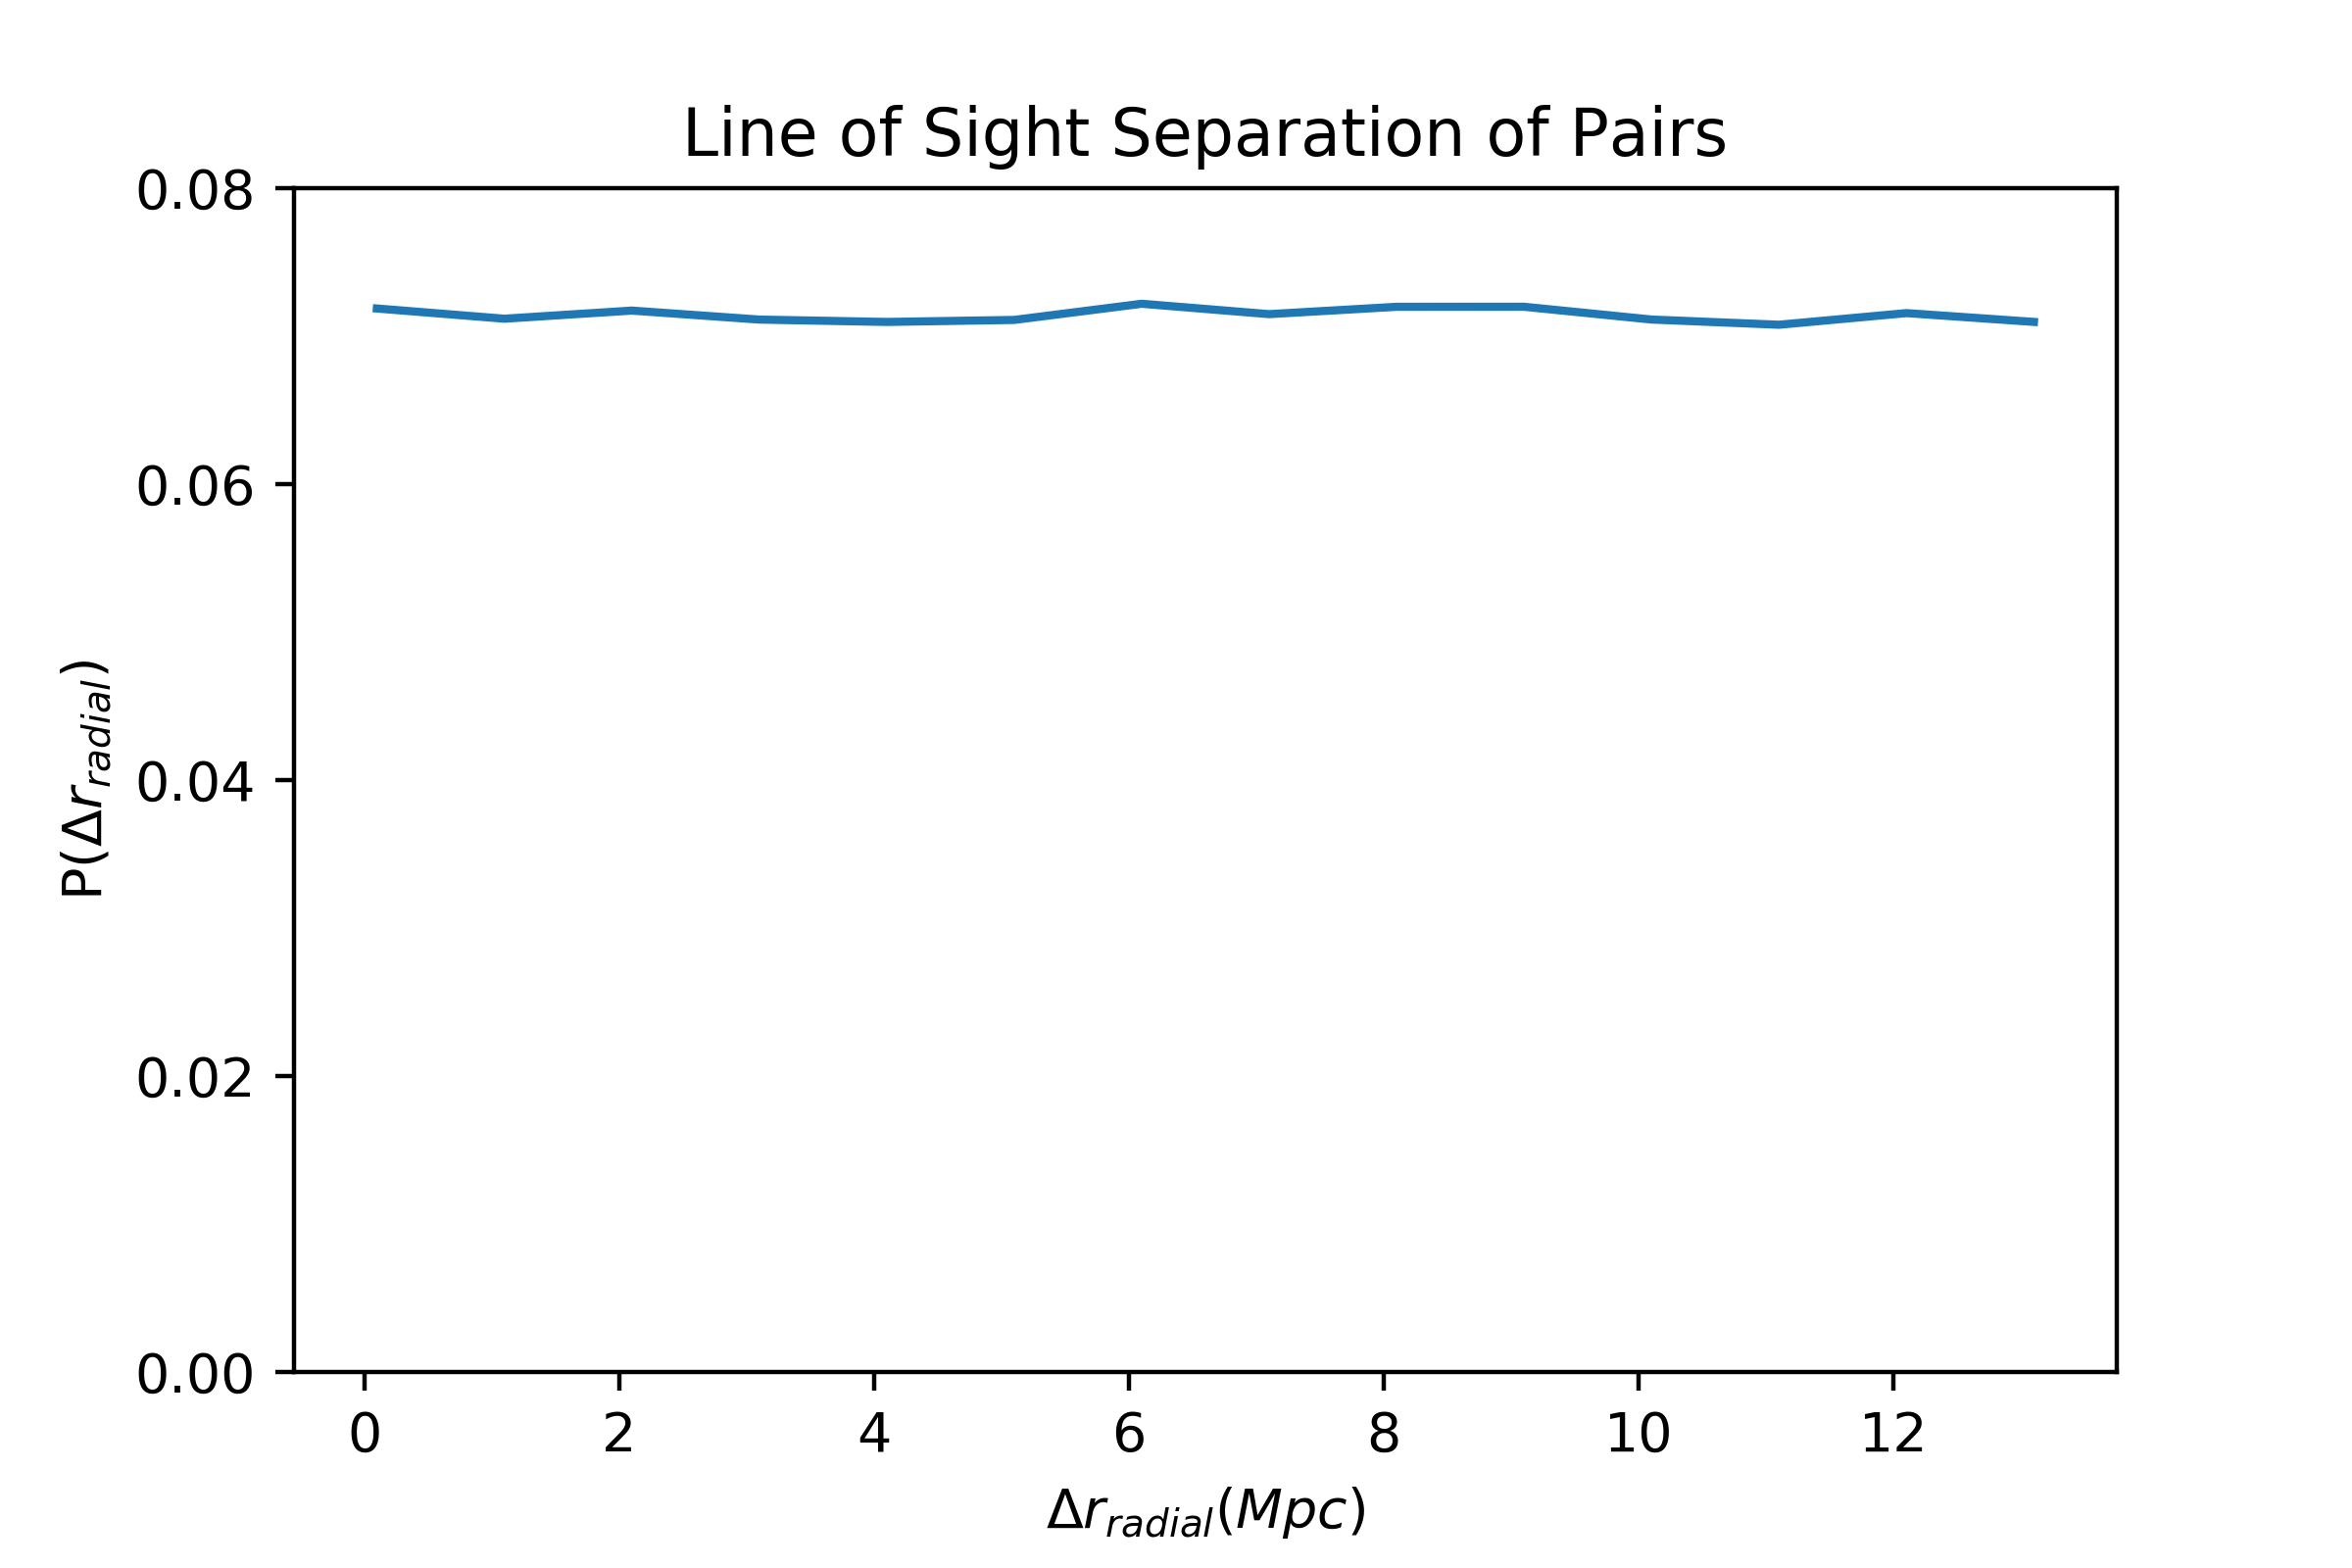
\includegraphics[width=0.6\textwidth , keepaspectratio]{/home/mitchell/Documents/masters/masters/thesis/Ver_2/figures/LOS_Separation.png}
\caption{Histogram of Line of Sight Separations of Galaxy Pairs. The distribution is relatively flat, with a minimum separation of $\SI{0}{\mega\parsec}$, and a maximum separation of $\SI{14.8}{\mega\parsec}$.}
\label{fig:physical:lineofsight}
\end{figure}


\begin{figure}[H]
\centering
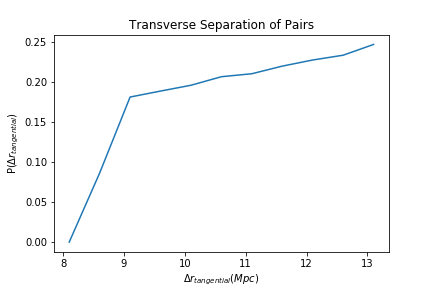
\includegraphics[width=0.6\textwidth , keepaspectratio]{/home/mitchell/Documents/masters/masters/thesis/Ver_2/figures/TRV_Separation.png}
\caption{Histogram of Transverse Separations of Galaxy Pairs. The distribution climbs steadily, with a minimum seperation of $\SI{8.85}{\mega\parsec}$ and a maximum separation $\SI{20.7}{\mega\parsec}$. }
\label{fig:physical:transverse}
\end{figure}

\par There are more pairs in higher transverse separation bins than in lower ones, which suggests that there will be a tendency to rescale pairs by smaller amounts in the algorithm. This will also effect the resulting halo shape, since pairs that are closer together will also by nature be scaled to larger effective halo sizes.  

The stacking procedure was performed on a Compton $y$-map produced from a combination of the South Pole Telescope SZ observing run, and the \emph{Planck} datasets. It made use of the $\SI{90}{\giga\hertz}$, $\SI{150}{\giga\hertz}$, and $\SI{220}{\giga\hertz}$ maps from SPT-SZ, and combined them with the $\SI{100}{\giga\hertz} - \SI{350}{\giga\hertz}$ and dust maps from \emph{Planck}, in the same manner as is described in \cite{2016ApJS..227...23C} (Bleem, in prep.). The algorithm for producing this map also took the half survey and half mission power spectra from \emph{Planck} as inputs. It minimised the contribution of the primary CMB, Cosmic Infrared Background (CIB), Instrumental, and Atmospheric sources as the primary sources of noise. 

We performed the stack on a map with a resolution of $\SI{0.25}{\arcmin}$ per pixel, but the effective resolution, after combining the beam sizes of the various raw data maps, is closer to $\SI{2}{arcmin}$, so there is likely some interpolation in the output, which would have introduced a source of noise.


Stacking these pairs returns an average $y$ map, which is shown in figure \ref{fig:physical:stack}. The signal is dominated by the contribution of the galaxy halos, and so these will need to be effectively subtracted in order to evaluate the significance of the filament signal. To the eye, there appears to be some residual signal in between the two halos, which has not been driven to zero as a result of the stacking process. 


\begin{figure}[H]
\centering
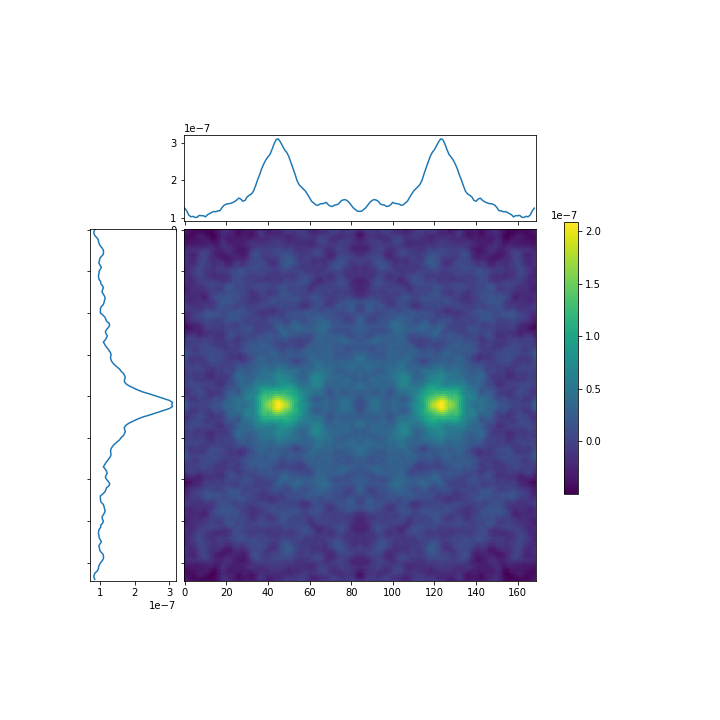
\includegraphics[width=\textwidth , keepaspectratio]{/home/mitchell/Documents/masters/masters/thesis/Ver_2/figures/Stack.png}
\caption{Stacked Image of galaxy pairs. The upper panel shows the slice through the centre of the stack. The left panel displays a vertical slice through the left halo, which by the mirroring procedurce, will be the same as the slice through the right halo.}
\label{fig:physical:stack}
\end{figure}

Once we have stacked the pairs, we perform our fit, as described in \ref{alg:analysis}. Beginning with our naive fit, we considered only a single halo, because the mirroring of the image essentially forces the two halos to look identical under this calculation. We also only consider the half of the halo that is on the other side to the filament, to prevent contamination from the filament. Doing so yields a halo shape shown in Figure \ref{fig:halo:single}.

\begin{figure}[H]
\centering
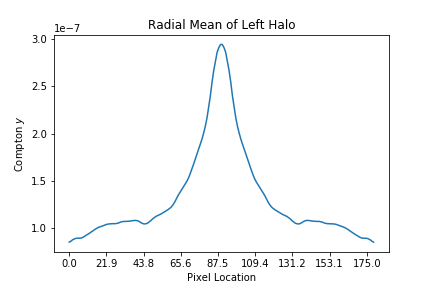
\includegraphics[width=\textwidth , keepaspectratio]{/home/mitchell/Documents/masters/masters/thesis/Ver_2/figures/halo_shape.png}
\caption{ Radial Mean of Left Halo from figure \ref{fig:physical:stack}. The shape of the halo does not appear to be gaussian in nature, perhaps owing to the uneven scaling depending on transverse separations. }
\label{fig:halo:single}
\end{figure}

Taking this halo shape, and assuming that there is some constant background signal of approximately $y = 1\times 10^{-7}$, we can combine this into our naive model, and find a measure of the residual filament. Assumig this constant background signal is functionally the same as taking a high bandpass filter of the stack. 


\begin{figure}[H]
\centering
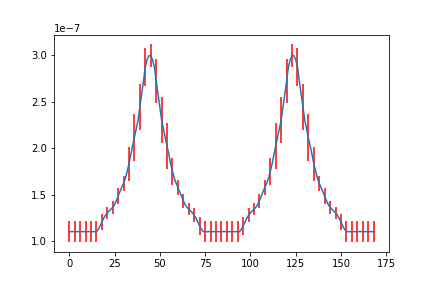
\includegraphics[width=\textwidth , keepaspectratio]{/home/mitchell/Documents/masters/masters/thesis/Ver_2/figures/halo_model_basic.png}
\caption{ Basic Halo Model, constructed from the radial mean of a single halo, with error bars given by the standard deviation of the halo in the same radial bins }
\label{fig:halo:basic_model}
\end{figure}

Figure \ref{fig:halo:basic_model} shows this model, with errors derived from computing the standard deviation of the radial halo in the same halo bins as the mean was calculated. Subtracting this from the slice through the halos gives us the graph shown in figure \ref{fig:halo:basic_filament}.

\begin{figure}[H]
\centering
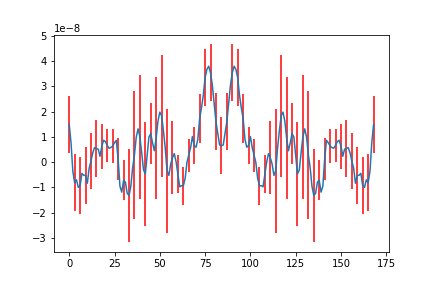
\includegraphics[width=\textwidth , keepaspectratio]{/home/mitchell/Documents/masters/masters/thesis/Ver_2/figures/filament_basic.png}
\caption{ Basic Filament Model, with filamentary residual shown between Pixel locations 60 and 110. }
\label{fig:halo:basic_filament}
\end{figure}

This naive calculation shows what is visible to the eye when looking at the stack in figure \ref{fig:physical:stack}, that there is some residual signal in between the two halos which should be from the filaments that connect the galaxy halos. The mean compton y parameter for this region is $\bar{y} \approx 1.9 \times 10^{-8}$, with a mean error of $8.31 \times 10^{-9}$. 



\par If we consider our more complex models in 1 dimension (along the central slice through both halos), and fit to our data, we get the results shown in figure \ref{fig:halo:complex_model}. All models were fit using standard definitions, and using a damped least-squares method known as the Levenberg-Marquardt algorithm.

\begin{figure}[H]
\centering
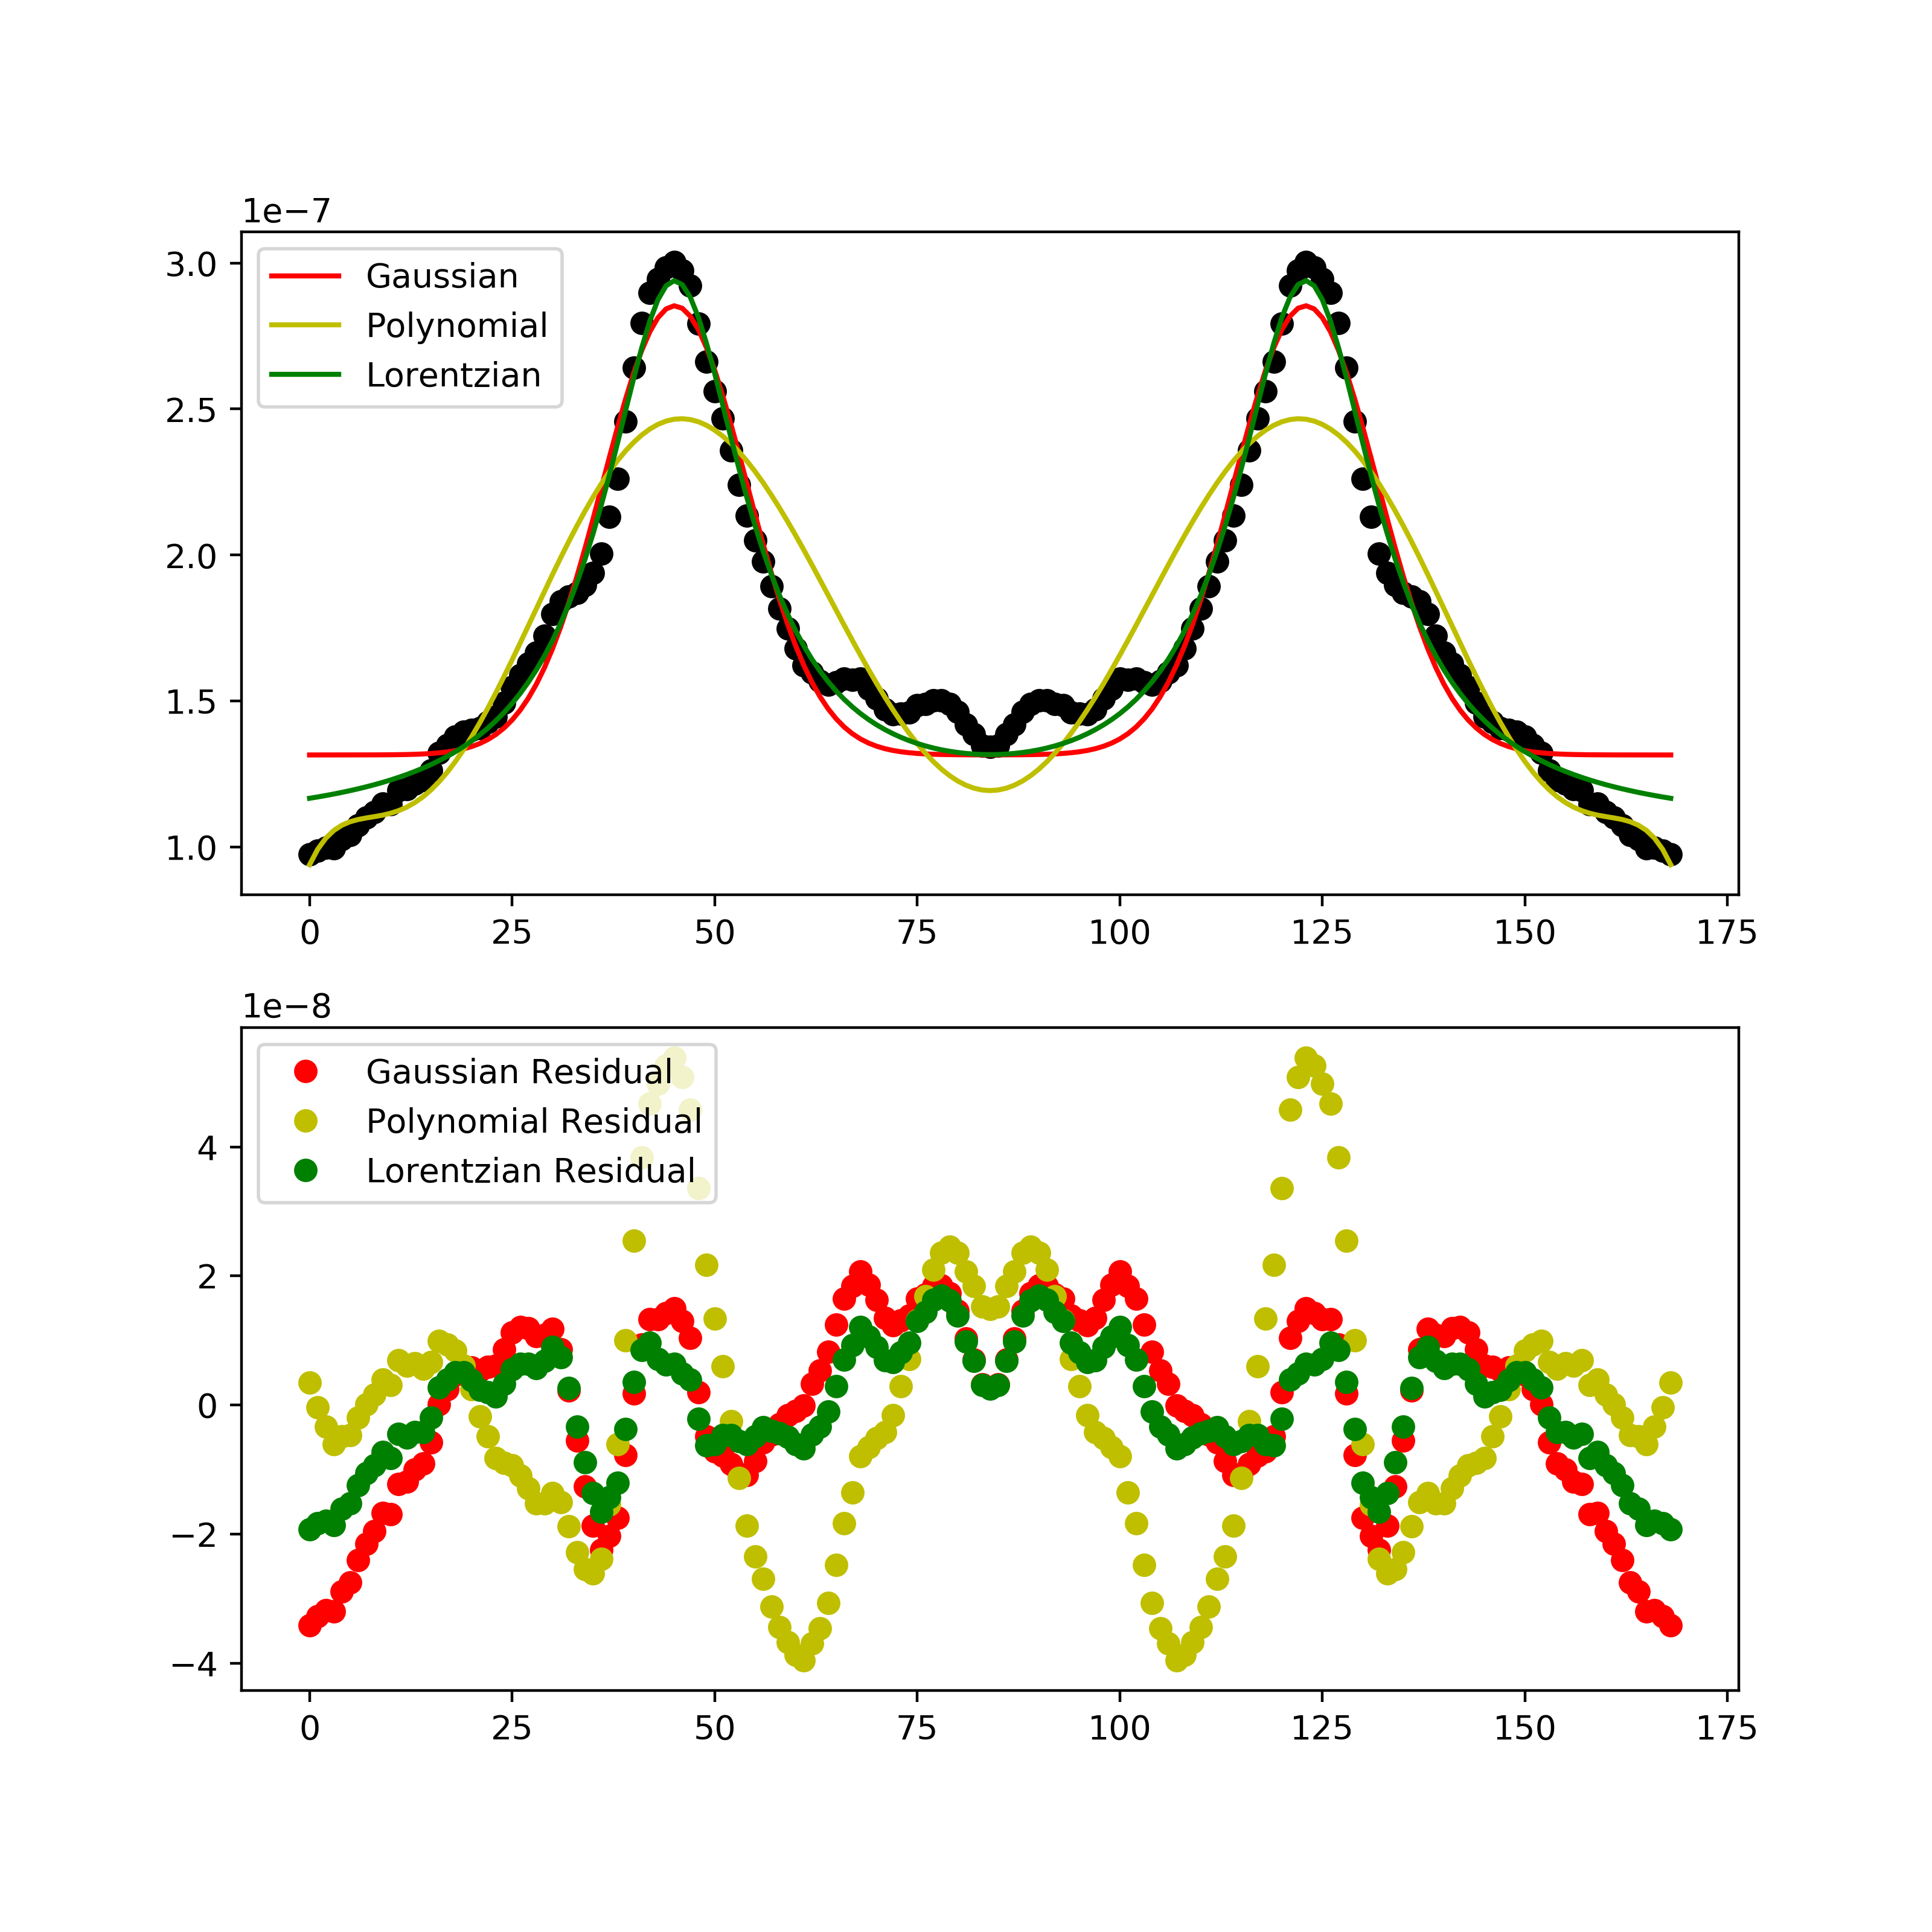
\includegraphics[width=\textwidth , keepaspectratio]{/home/mitchell/Documents/masters/masters/thesis/Ver_2/figures/halo_model_complex.png}
\caption{ Multiple Halo Models fitted to Central Slice of Figure \ref{fig:physical:stack} }
\label{fig:halo:complex_model}
\end{figure}

These are noticably worse than our simple model. The polynomial fit doesn't subtract the halos properly, so we discard it here. The gaussian model does subtract most of the halos away, but the left-over signal is significantly lower, with a mean residual Compton $y$ of $\tilde{y} \approx 8.68 \times 10^{-9}$. The fact that the gaussian models fail to match the curves at the centres of the halos does suggest that it is a poor model.

\par Given the apparent shape was non-gaussian, we applied a Lorentzian fit to the shape of the halos. This fit the halo shapes much better, and dies away much quicker than the gaussian model, but also removes more of the signal we are looking for. It is possibly that this is simply the best fit for the algorithm we have implemented, and a change in our process would result in another model fitting better. It is also incredibly difficult to explain why the halo shape would be lorentzian physically, further reinforcing the idea that it is the result of introduced scaling effects in the algorithm. 

\par Considering that the model of the halo seems to have a non-gaussianity to it, we performed a number of two dimensional model fits to our two dimensional image of the stacks. The models we chose to fit to the data were 
\begin{enumerate}[label=(\Roman*)]
\item 4 Independent Gaussians \label{2D:model:1}
\item 2 sets of 2 coupled Gaussians \label{2D:model:2}
\item 4th order polynomial \label{2D:model:3}
\item Spherical Gaussians \label{2D:model:4}
\end{enumerate}

We chose to use variations of multiple gaussians in order to take into account the distorted shape of the halos. In model \ref{2D:model:1}, we allow 4 gaussians to vary independantly. In model \ref{2D:model:2}, we couple the underlying gaussians together, so that one pair of them will extract the spread of the halo, and another will extract the height. We chose model \ref{2D:model:3} to maintain consistency with our fit from the simple 1D case. In model \ref{2D:model:4}, we force the gaussians to contain our assumption of spherical halos. 

\begin{figure}[H]
\centering
\includegraphics[width=\textwidth , height=\textheight , keepaspectratio]{/home/mitchell/Documents/masters/masters/thesis/Ver_2/figures/2D_data_fitting.png}
\caption{ Multiple Halo Models fitted to 2D array of Figure \ref{fig:physical:stack} }
\label{fig:halo:2D_complex_model}
\end{figure}

When we look at these models, none of them seem to appropriately subtract the halo contributions. 
\par Model \ref{2D:model:1} appears to do the best, removing the majority of the halo, and leaving behind a reasonably strong signal where we would expect to see a filament. What is noticable however, is that the right halo in the model is distorted along some diagonal axis, which is strange, given the data that is being fitted to has been made symmetric about two axes. This results in greater subtraction in the residual of the right halo than the left, and so introduces some error in our measurement of the filament. It also leaves a very large amount of signal in the central region, in what looks like a hourglass shape. It is unclear if this is indicative that filaments don't necessarily link galaxies in a straight line, or if it is an artefact of the mirroring process.
\par If we correct for the perceived issues with the first model, model \ref{2D:model:2} forces the gaussians into sets of two, which each obey the same statistics, therefore accounting for the mirroring in the image. This form of the model does succeed in extracting nearly all of the halo, but leaves so much residual signal everywhere that it looks like we are extracting residual baryons from areas surrounding the galactic halos. 

\par Unfortunately, \ref{2D:model:3} extracts too much of the signal, and not enough of the halos. This may be due to the way that the model is being fit to the data. Since the data is symmetric about the central $x$ axis, the model fitting will see the same value on both sides of the masked area. This forces the fit to assume that the data holds the same value across the masked area, removing the possibility that the halos fall away, and so preventing us from detecting the filament signal. If we perform the fit on the whole array of data, the polynomial overfits the data, and subtracts the entirety of the filament signal anyway. The current fit doesn't subtract the whole halo signal either, meaning that the data isn't being fit properly with the current mask. 
\par Model \ref{2D:model:4} also extracts too much of the filament signal. It appears that forcing the spherical shape of the halos causes too much crossover in the modelled halos. This effectively leaves us with no filament signal, allowing us to discard this model. Doing so does raise some interesting points however, regarding our assumption of spherical symmetry. 


\par These two dimensional models do not perform as well as the one dimensional ones, either in terms of accuracy or strength of signal. This is likely due to the increased amount of noise in the two dimensional image, as opposed to the one dimensional slice. The higher resolution in the $y$ map we use could also be introducing this higher level of noise, since it would not necessarily be smoothed out by the detector beam. 

\par The results for all models which are considered sensible are included in Table \ref{table:results}. 

\begin{table}[H]
\centering
\begin{tabular}{||c c c c||} 
 \hline
 Model & Mean Residual $y$  & Error & Sigma\\
 \hline\hline
 Radial Mean 1D Fit & $2.5\times 10^{-8} $ & $\pm 7.72 \times 10^{-9}$ & $3.24$\\
 \hline
 1D Gaussian Fit & $1.29\times 10^{-8} $ &  $\pm 6.29 \times 10^{-9}$ & $2.05$\\
 \hline
 2D Model 1 & $1.38\times 10^{-8}$ & $\pm 1.77 \times 10^{-8}$ &  - \\
 \hline 
 2D Model 2 & $0.82 \times 10^{-9} $ &  $\pm 1.59 \times 10^{-8}$ & - \\
 \hline \hline 
\end{tabular}
\caption{Results for residual mean filament for various fitting methods }
\label{table:results}
\end{table}

Given the necessity of accounting for both halo contributions at all points in the stack, we hold that the best result to quote is the 1D gaussian fit. Our fiducial value of the average Compton-$y$ of the filament is 
\begin{equation}
\boxed{\bar y = 1.29 \times 10^{-8} \pm 6.29 \times 10^{-9}}
\end{equation}
\section{Null Tests}
\subsection{Un-Physical Pairs}
We constructed a catalogue of unphysical pairs from the galaxies contained in both the SPTpol and DES survey footprints, with radial separations between $\SI{100}{\per\h\mega\parsec}$ and $\SI{200}{\per\h\mega\parsec}$, and transverse separations between $\SI{6}{\per\h\mega\parsec}$ and $\SI{14}{\per\h\mega\parsec}$. 

\begin{figure}[H]
\centering
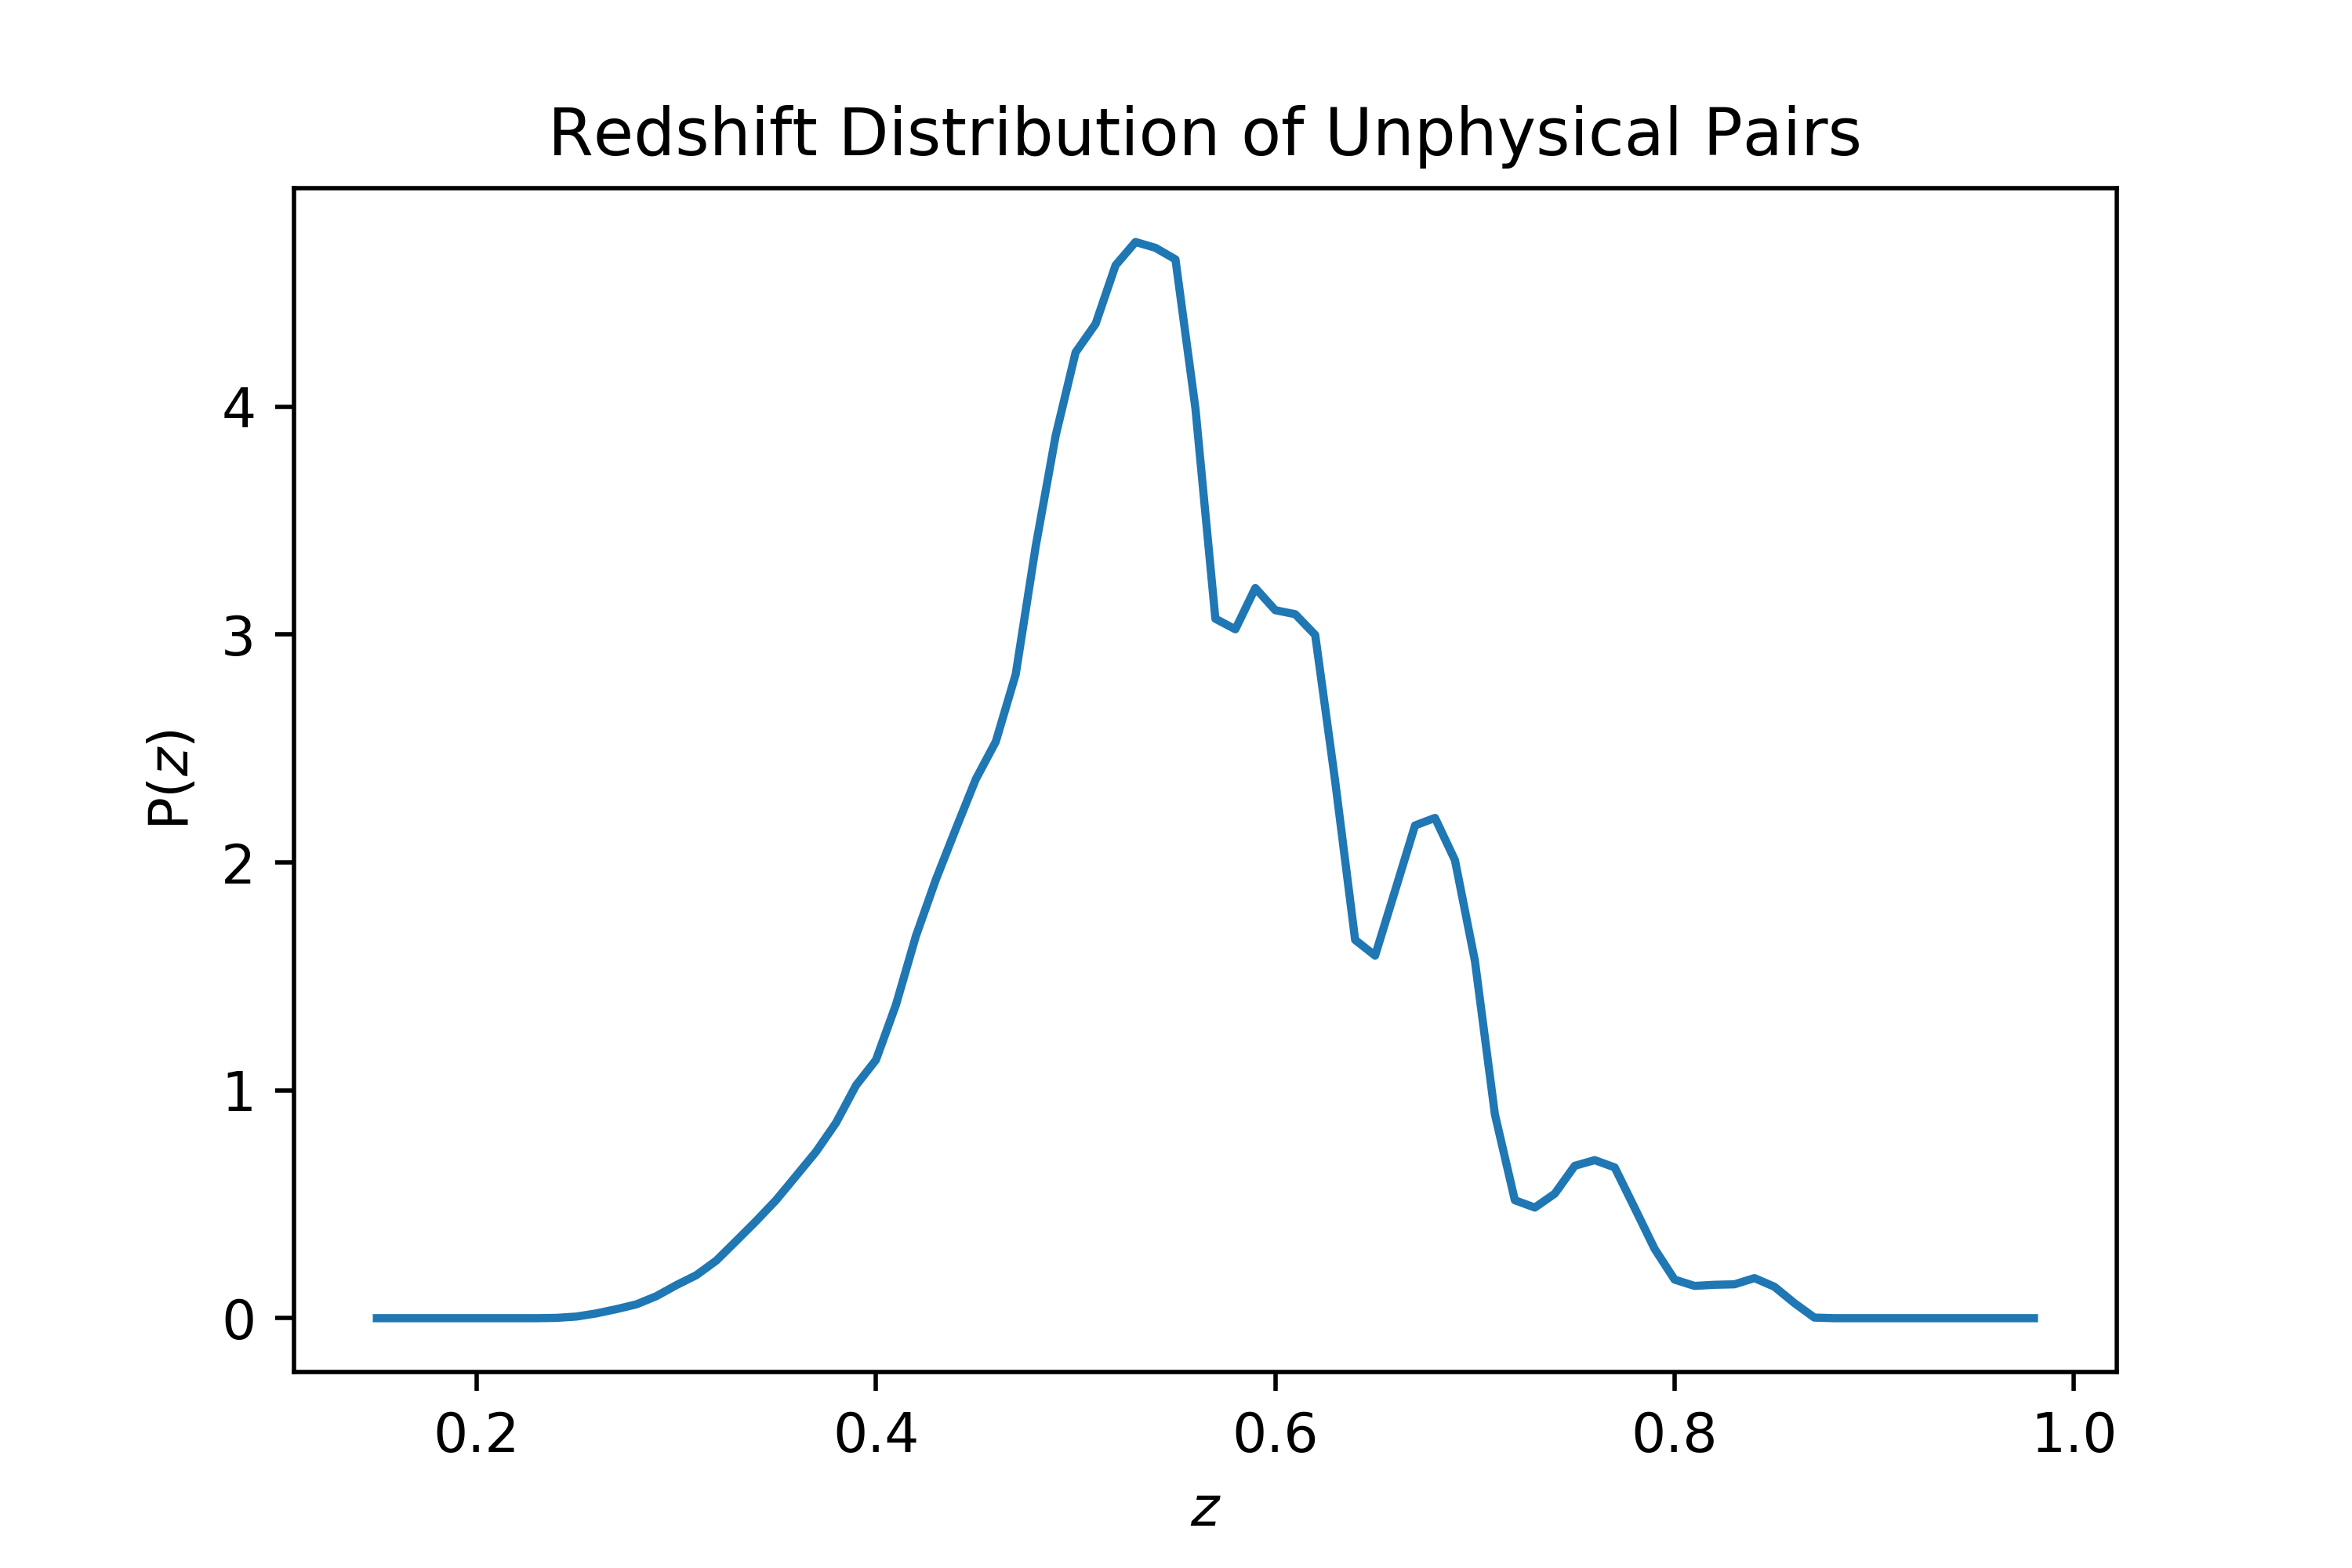
\includegraphics[width=0.6\textwidth , keepaspectratio]{/home/mitchell/Documents/masters/masters/thesis/Ver_2/figures/UnPhysical_Redshift_Distribution.png}
\caption{Redshift Distributions of Unphysical Pairs. The pairs range from redshifts $z\approx0.24$ to $z\approx0.87$, with a mean redshift of $z\approx0.55$. When compared to the physical pairs, this set has a higher mean redshift, and more pairs in higher redshift bins.   . The distribution of physical pairs is overlaid in red.}
\label{fig:unphysical:redshifts}
\end{figure}
As can be seen in figure \ref{fig:unphysical:redshifts}, the distribution of redshifts is generally skewed towards higher redshifts than for the physical pairs. This is likely due to the inherent errors assosciated with the photometric redshifts in the DES redMaGiC survey. Lower redshifts are more likely to be more precise, since the photometric errors for redshift are given by $\Delta z= 0.01(1+z)$, and so be excluded by the line of sight cuts. The other effect which may influence this is the fact that there are far more pairs in the unphysical dataset than in the physical dataset. 


This produced a set of unphysical pairs containing $\sim 670,000$ pairs, with a mean line of sigh separation of $\SI{220}{\mega\parsec}$, and a mean transverse separation of $\SI{12.5}{\mega\parsec}$.


\begin{figure}[H]
\centering
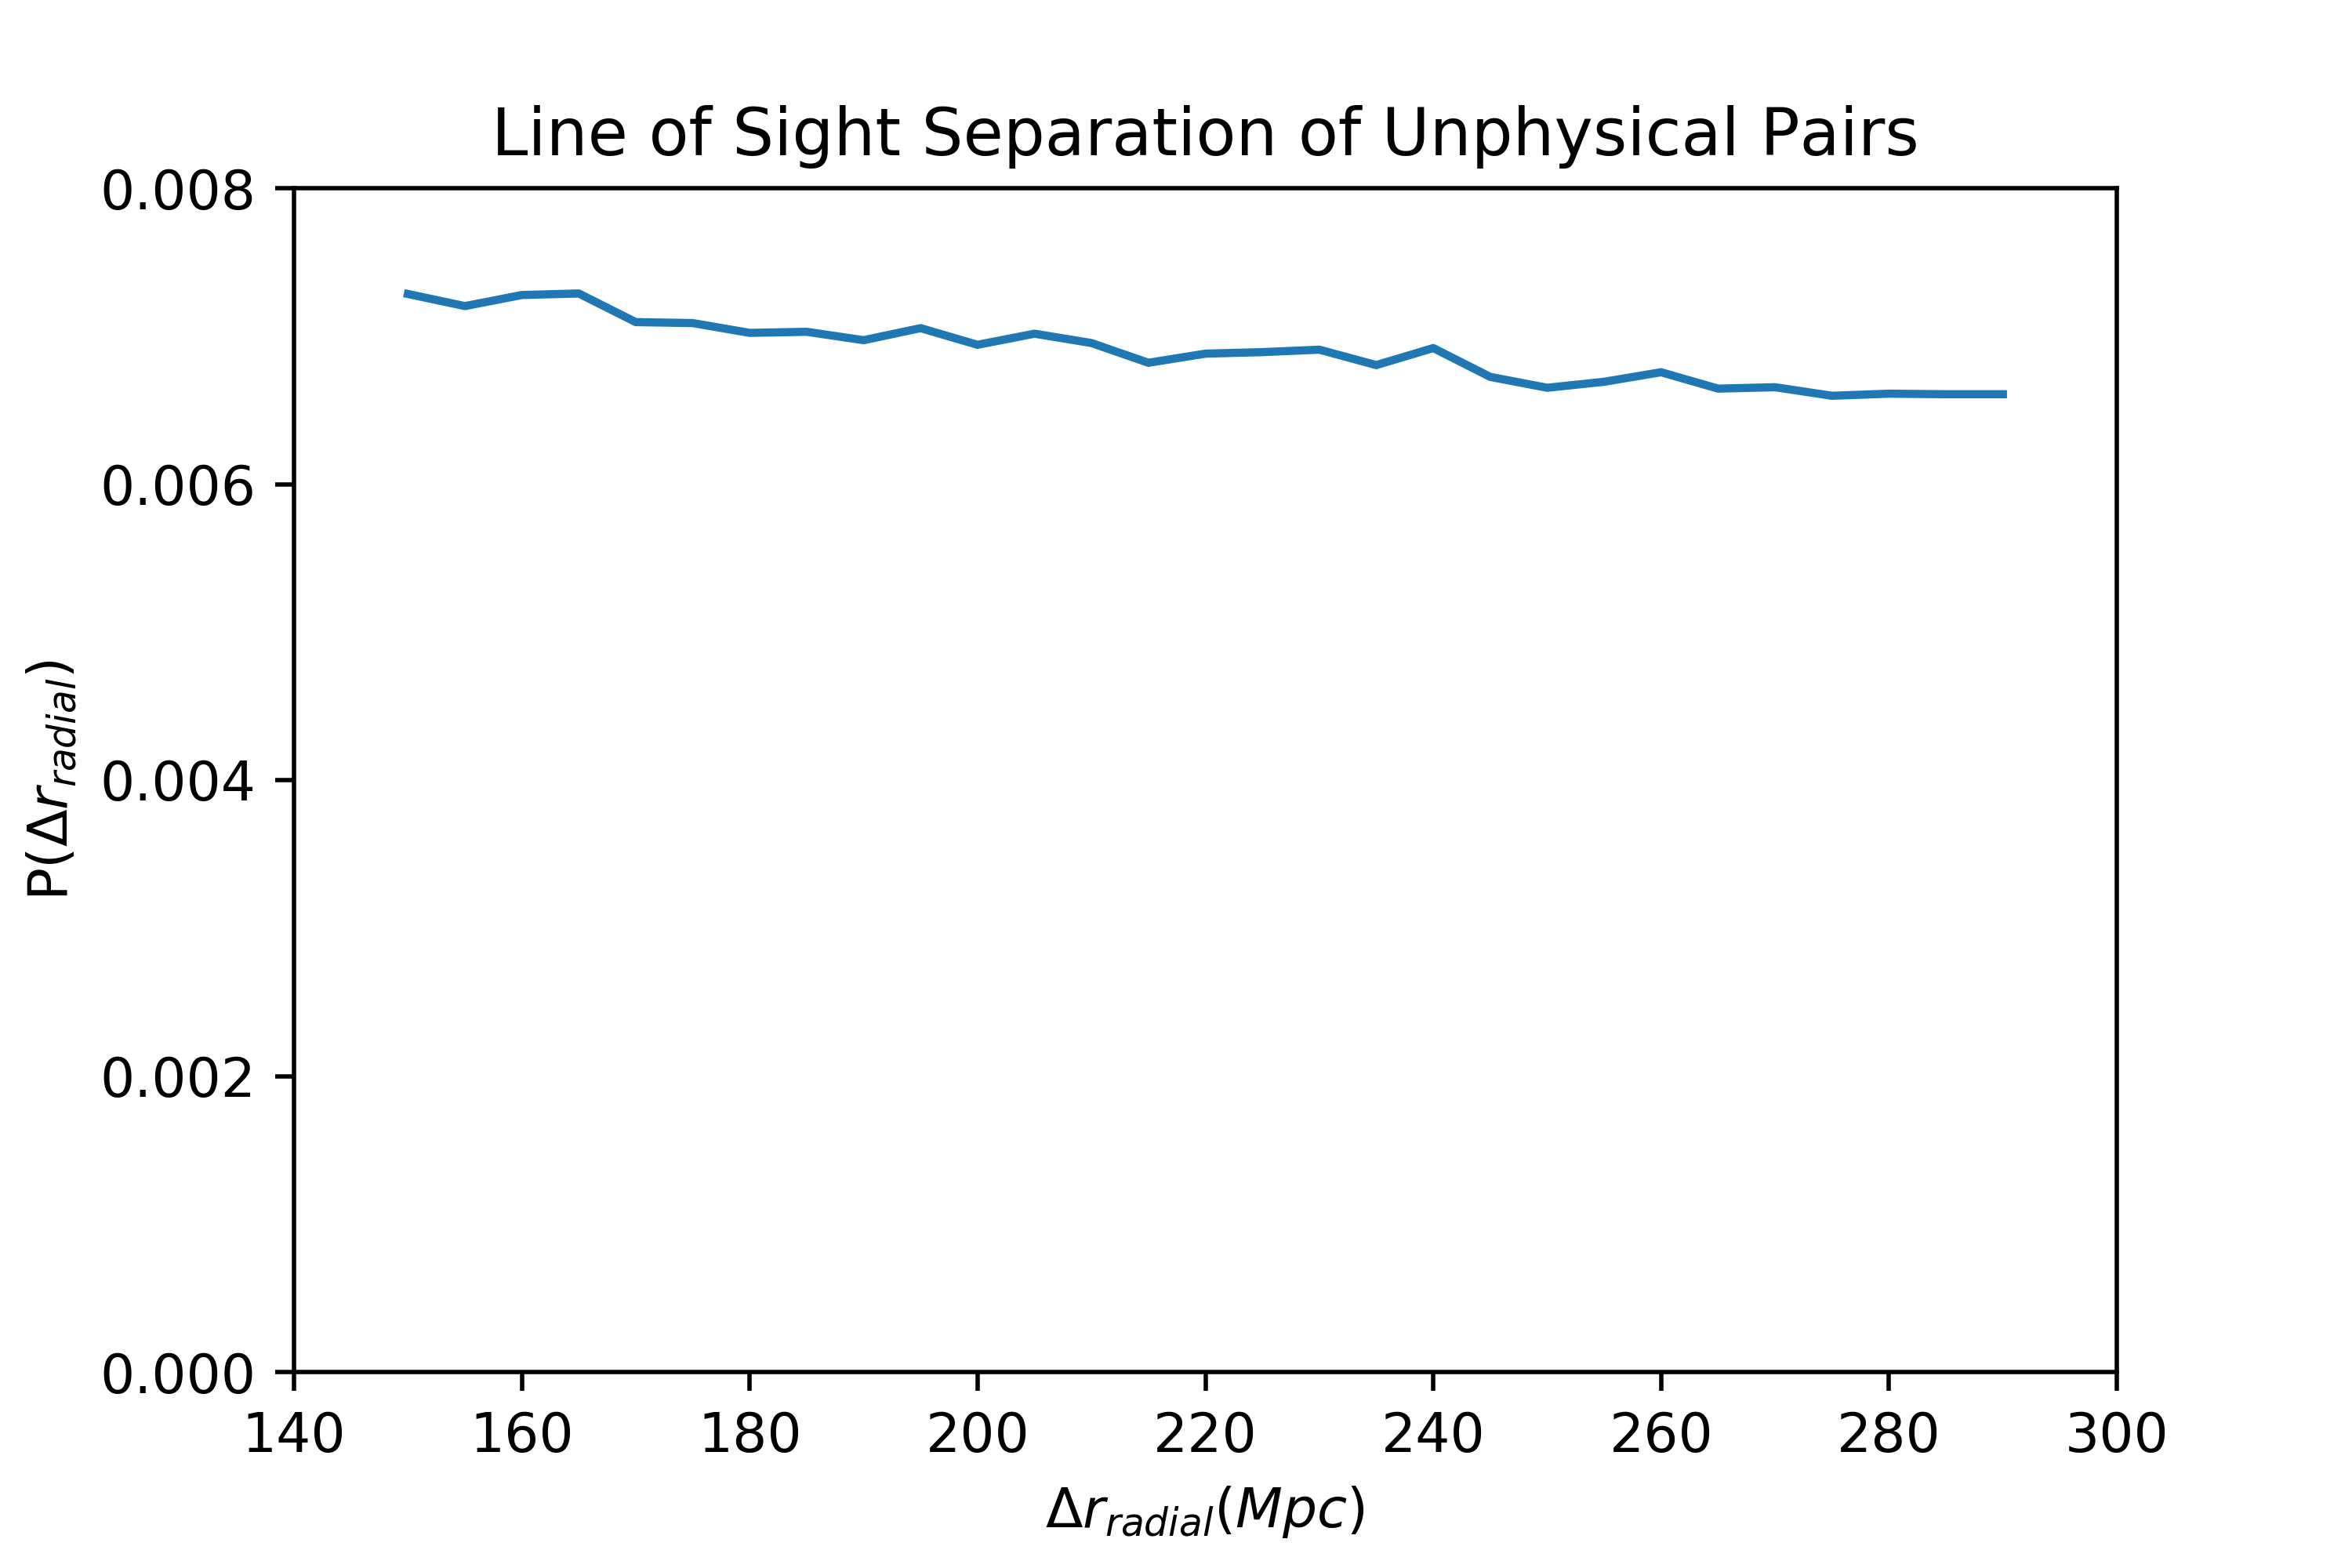
\includegraphics[width=0.6\textwidth, keepaspectratio]{/home/mitchell/Documents/masters/masters/thesis/Ver_2/figures/UP_LOS_Separation.png}
\caption{Histogram of Line of Sight Separations of Unphysical Galaxy Pairs. The distribution is relatively flat, with the same shape as the physical pairs, a minimum separation of $\SI{147}{\mega\parsec}$, and a maximum separation of $\SI{295}{\mega\parsec}$.  }
\label{fig:unphysical:lineofsight}
\end{figure}

The choice was made to consider unphysical pairs with a line of sight separation in excess of $\SI{100}{\per\h\mega\parsec}$ because at large redshifts, the errors assosciated with the photometric redshifts can place a very large range on the possible distance to a given galaxy, and we want to be very careful to exclude galaxy pairs that might have a connecting filament between them. 

\begin{figure}[H]
\centering
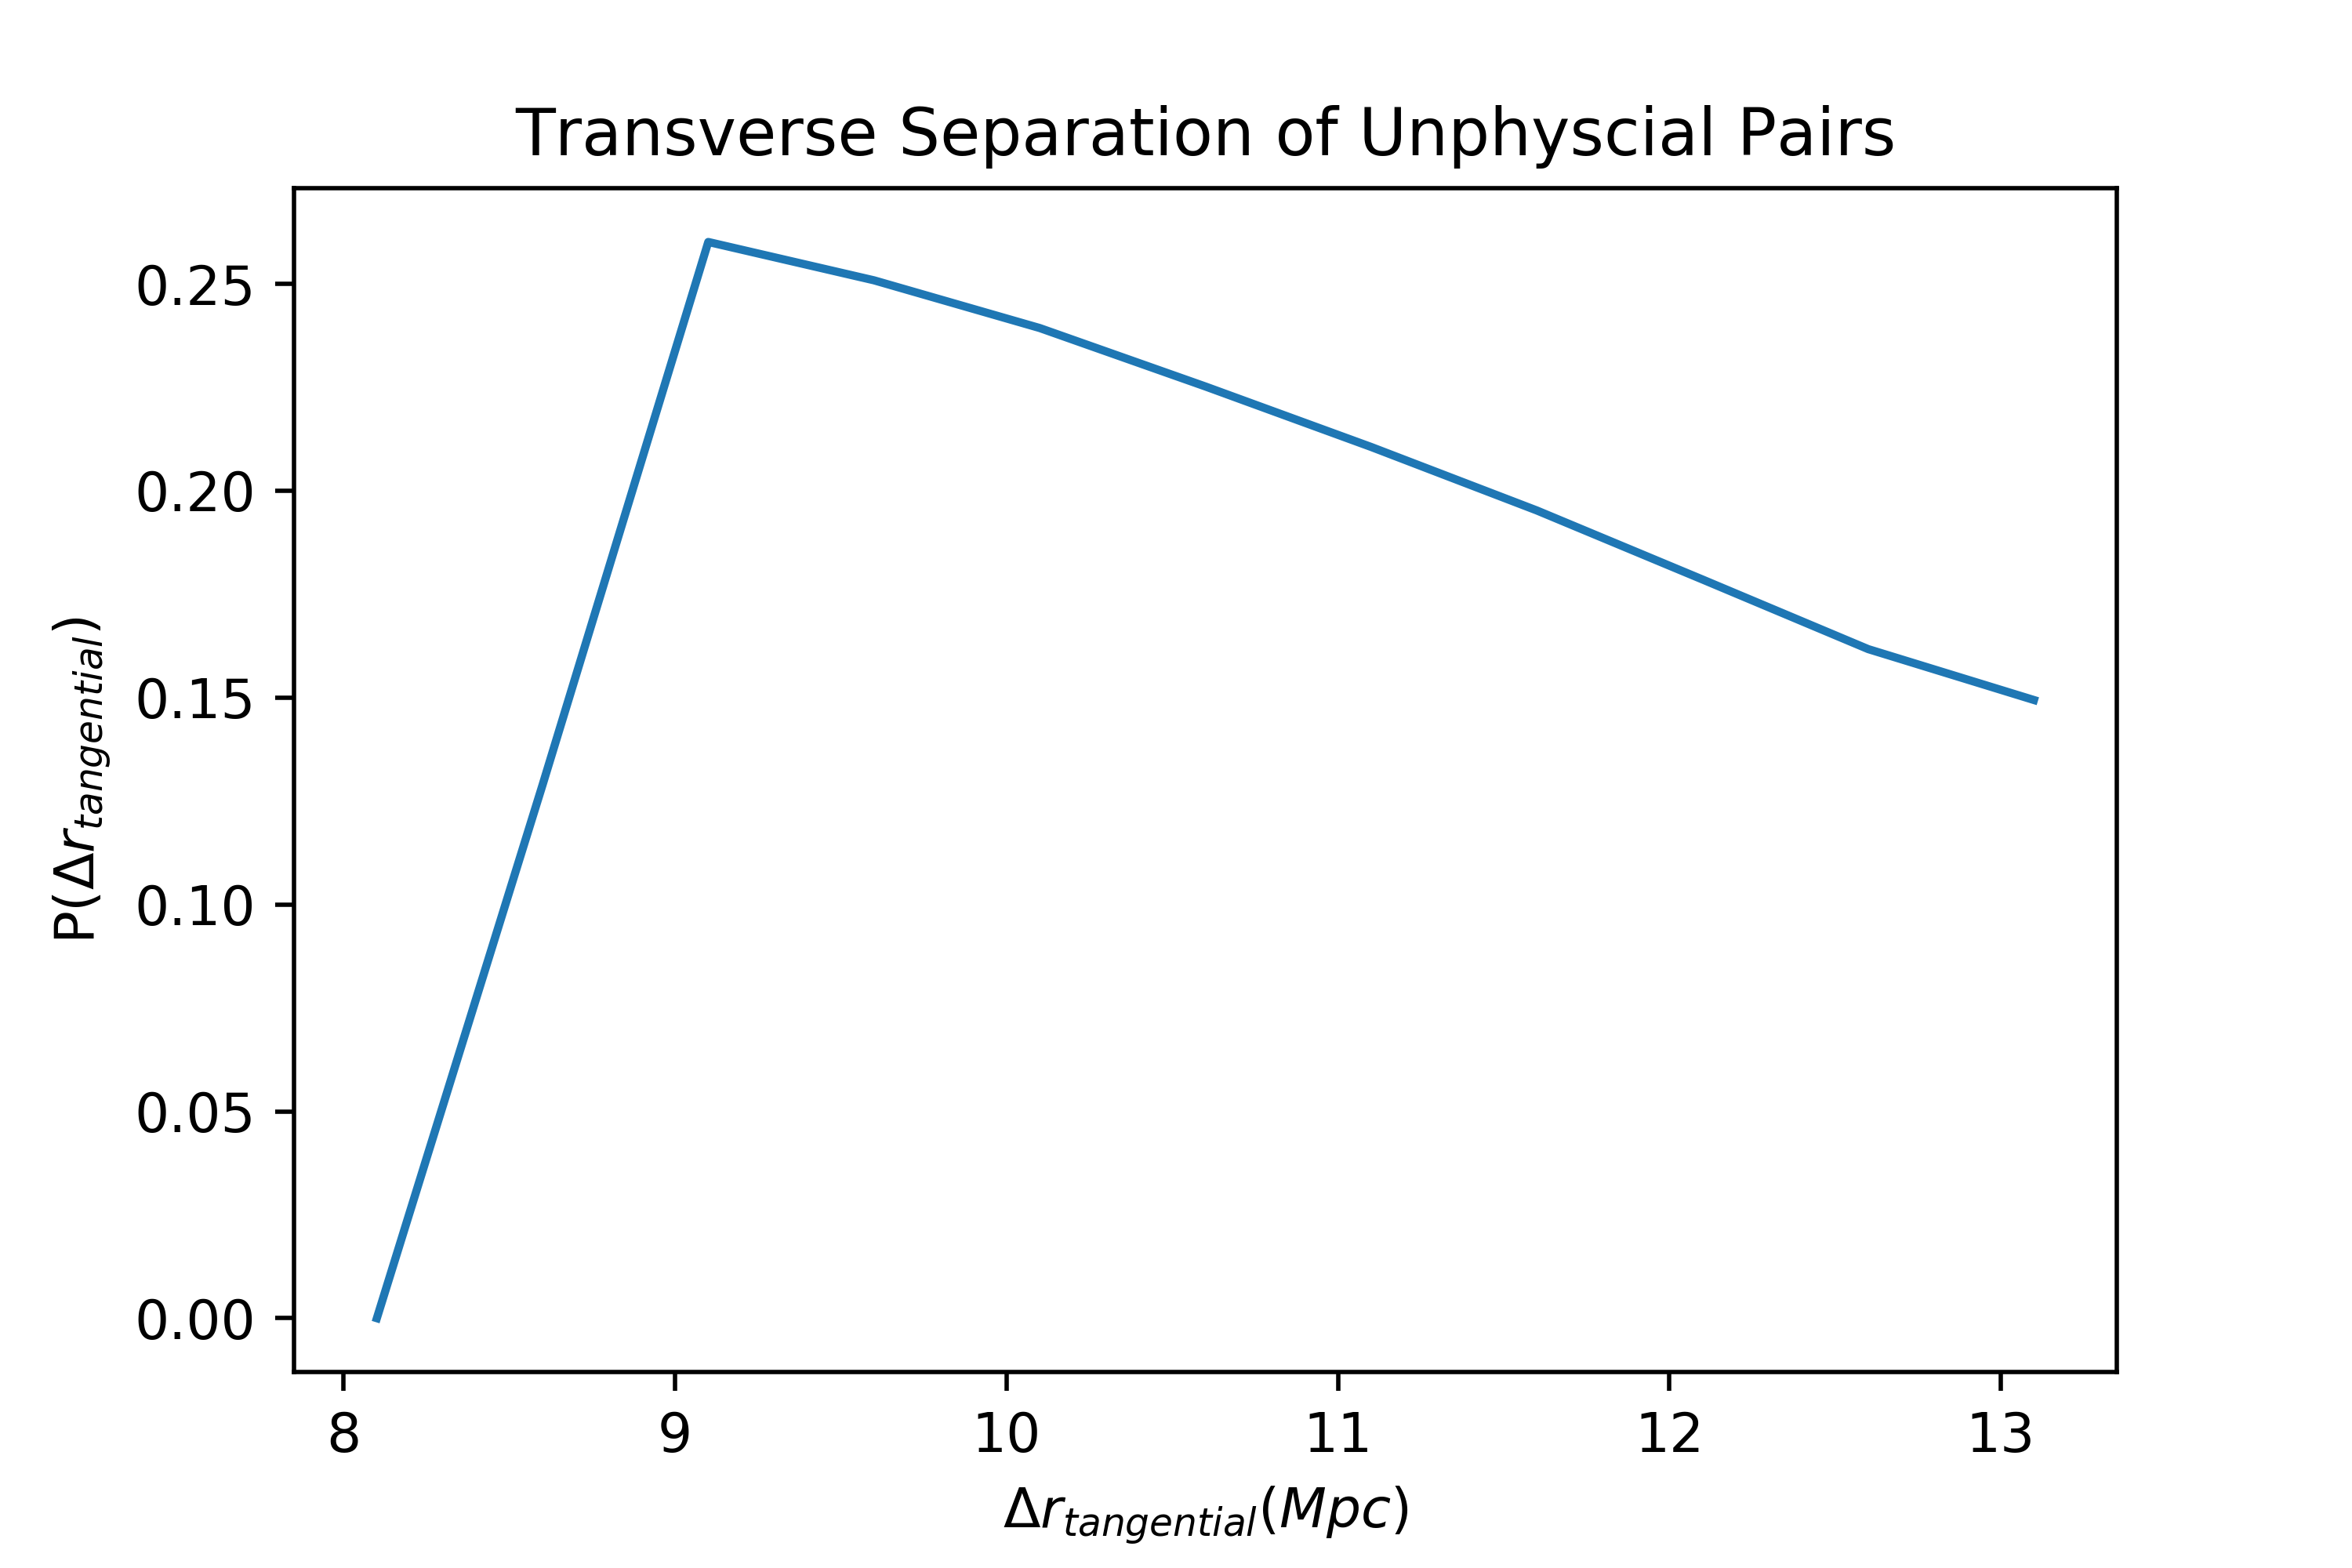
\includegraphics[width=0.6\textwidth  , keepaspectratio]{/home/mitchell/Documents/masters/masters/thesis/Ver_2/figures/UP_TRV_Separation.png}
\caption{Histogram of Transverse Separations of Unphysical Galaxy Pairs. The distribution is relatively flat, with a minimum seperation of $\SI{8.85}{\mega\parsec}$ and a maximum separation $\SI{20.7}{\mega\parsec}$. This has the same overall shape as the physical pairs data set, except the relative population in the higher separation bins decreases, rather than increases.}
\label{fig:unphysical:transverse}
\end{figure}

Performing the stacking procedure on the unphysical dataset gives the stack shown in figure \ref{fig:unphysical:stack}. To the eye, in both the 2D slice and the 3D colour map, it appears that there is less filamentary signal than for the physical pairs. 

\begin{figure}[H]
\centering
\includegraphics[width=0.8\textwidth , keepaspectratio]{/home/mitchell/Documents/masters/masters/thesis/Ver_2/figures/UnPhysical_Stack.png}
\caption{Stacked Image of Unphyiscal pairs.}
\label{fig:unphysical:stack}
\end{figure}

If we fit the two halos for gaussian profiles (shown in figure \ref{fig:halo:basic_filament}) , along with some constant offset, we can see very clearly that there appears to be no residual signal left. The mean of this residual is $3.48 \times 10^{-18}$, with a variance of $1.13 \times 10^{-16}$, which is consistent with a zero measurement. 


\begin{figure}[H]
\centering
\includegraphics[width=\textwidth , keepaspectratio]{/home/mitchell/Documents/masters/masters/thesis/Ver_2/figures/unphysical_halo_fit.png}
\caption{Gaussian Fit to Unphysical Pairs}
\label{fig:unphysical:fit}
\end{figure}

\subsection{Random Stack}

Performing a stack on a set of pseudo-randomly selected slices of the CMB, with the same galactic latitude as the physical pairs, we produced a stack like the one shown in Figure \ref{fig:random:stack}. This has no discernable structure, except for the small circular signal in the centre of the map. This is likely due to the rescaling effect still rescaling the CMB as if it were trying to align pairs. Because the angle that the pairs need to be rotated by should be evenly distributed, there should be some level of correlation in the stack, in a circular structure where we would otherwise expect a filament to be. 

\begin{figure}[H]
\centering
\includegraphics[width=\textwidth , keepaspectratio]{/home/mitchell/Documents/masters/masters/thesis/Ver_2/figures/Rand_Pos_Stack.png}
\caption{Stack of pseudo-random slices}
\label{fig:random:stack}
\end{figure}



	% Reproduction of the shear signal
	% Effect of varying spatial and velocity resolution
	% Recovery of the shear signal from real data
	% Discussion of problems with the results

	%\include{Prob_of_lensing}
	
	% Analysis of lensing probability


  %\include{Science_for_SKA}

	% Need for better quality data
	% Probability of lensing out to a given z
	% Science case for SKA based on this and results stuff
	
	%Further work:
	%app to real gals
	%complimentarity with current methods
	%h alpha 
	%prob of lensing
	%science case for SKA
	%fit for centroid later

 	\chapter{Discussion and Conclusion}

\section{Discussion}
Our measure of the Compton $y$ parameter in the filament of $\bar{y} = 1.29 \times 10^{-8}$ at $2.05 \sigma$, is comparable to similar work done by \cite{2019A&A...625A..67T} (refered to as T17), and by \cite{2019A&A...624A..48D} (refered to as G17).

\par T17 found 262,864 galaxy pairs at redshifts $z<0.4$ using the Sloan Digital Sky Survey LRG catalogue, detecting a mean Compton parameter of $y \approx 1 \times 10^{-8}$ in the \emph{Planck} $y$ map at a $5.3\sigma$ confidence level. 

\par G17 found 1,020,334 galaxy pairs in a redshift range $0.43 < z < 0.75$ using the Sloan Digital Sky Survey CMASS catalogue, detecting a mean Compton parameter of $y \approx 0.6 \times 10^{-8}$ in the \emph{Planck} $y$ map at the $5.1\sigma$ confidence level. 

\par The two catalogues used by T17 and G17 are both independent of each other, since they cover different redshift ranges, but the similar detection levels, and detection strengths lends strong evidence to the existence of filaments which can be detected by tracers in the CMB. 

\par G17 directly calculated the baryon fraction from their residual Compton $y$ parameter as being $\sim 0.3 \Omega_b$. Our measurement of the Compton $y$ parameter is much higher than theirs, but there are a number of factors which differentiate our measurement from previous work. 

\par Previous calculations operated on the \emph{Planck} $y$ map only, which has an effective beam size of $\SI{10}{\arcmin}$, which effectively acts to convolve any signal contained in the map. This introduces some error into the measurement, but mostly acts to smooth out the $y$ map. The choice has to be made then, to not consider pairs that are too close to each other, because if they fall within the width of the beam, they will be functionally indistinguishable, and it will be impossible to separate the contributions from their halos and the filament. The $y$ map we are using was produced primarily from the \emph{SPT-SZ} detection maps, and has a significantly smaller effective beam size than the \emph{Planck} map alone, of $\SI{2}{\arcmin}$. This means that we can make a choice to include more close pairs than previous work, because they will be able to be effectively resolved in our $y$ map. 

\par There are also a number of significant differences between galaxy catalogues used by previous works, and this one. Both T17 and G17 made use of galaxy surveys with spectroscopic redshifts, as opposed to photometric redshifts. Spectroscopic redshifts are taken by directly measuring spectra for a given galaxy, and identifying known spectral features in it. This makes it very easy to get an accurate measure of the redshift of a galaxy, but the process of producing a spectrum takes a long time, since it requires receiving enough photons to fill an entire spectrum. For this reason, many surveys make the choice to use photometric redshifts instead.

\par Photometric redshifts fundamentally measure the brightness of objects through various filters, and fits those to template objects with known redshifts. Often, this involves building a catalogue of spectroscopic objects from which a model can be constructed. Each new set of photometry is then applied to this model to detemine the redshift of each object. This is a much quicker process, because it doesn't require long integration times in order to get an measure of an objects redshift. Because it requires fewer photons to make a direct detection, it also allows for the calculation of redshifts for much dimmer objects than for spectroscopic redshifts. 

\par Because the algorithm assumes that the redshifts are accurate, this introduces some measure of spread in the bounds on the line of sight separations in the galaxy pairs. Ultimately, this doesn't have too large an effect on the measurement, because if a galaxy pair doesn't contain a filament, it will simply not contribute to the underlying signal, but will contribute to the halo signals.  

\par It also seems that we haven't managed to successfully construct galaxy halos that take the form of gaussians from our list of galaxy pairs. This may be due to the uneven distribution of galaxy pair separations on the sky, so we could possibly correct for this by selecting an even distribution of transverse separations. The other possible correction that could be made here is to sample more pairs, over a larger area. This would drive the distribution of scales closer to sampling from a gaussian by the central limit theorem, and so hopefully drive the shape of the rescaled halos to the same distribution. 

\par One possible method of mitigating this effect is to make better use of the null tests when analysing our physical pairs. This could be done by constructing sets of unphysical pairs which contain the same number as the physical set. We could then subtract the unphysical stack from the physical stack. Doing this for a number of different bundles of unphysical pairs would allow us to take an average, and hopefully model the overarching halo structure as subject to our analysis pipeline. 

\par The significance of the signal detected is lower than that of that of previous work ($\sim 2\sigma$ c.f. $\sim 5 \sigma$), due to the unreliability of our modelling, and the uncertainty introduced by uneven scaling factors. Despite this, the higher reading for our Compton $y$ parameter is considerably higher than previous work, which we attribute to the higher precision of the $y$ map we are using. 

\par We performed our fit initially on the SPTpol footprint only, due to the expense in computation when constructing galaxy pairs. With less than a sixth of the original catalogue, over 700 000 pairs were produced. For the sake of edification, the pairing algorithm was run on the full SPT-SZ footprint, and it produced $\sim 5.8$ million physical pairs, and over $15.5$ million unphysical pairs. With this number of pairs, even the stacking algorithm becomes compuationally expensive. 

\subsection{Further Work}

\par Further work can be done to strengthen the conclusions drawn by this work. Improvements in model construction, and refinement of the algorithm are possible 

\par Further work can apply this algorithm to other data sources. Any data source which acts as a tracer for large scale structure with known statistical information, can be used, since the algorithm doesn't discriminate based on input data type. This process was initially developed for $\kappa$ convergence maps \citep{2016MNRAS.457.2391C}, but it can equally be applied to the other form of \sze, Kinetic \sze , which acts as a tracer for bulk velocities in the intervening structure. 

\par All previous work has been done with single data sources, but performing it with multiple allows for calculations of cross correlations between independant data sources, which have some major advantages over single source detections. Many of the systematics between the data types will be uncorrelated, and so improve the quality of our signal, whilst driving the noise assosciated with the detection down. 

\par As it stands, there is strong evidence for the existence of galactic filaments from several independant teams. This work is the first to perform it with a high resolution CMB dataset, and provides strong support for previous measurements. 

	% Shown it can be done
	% Will be detectable when high enough resolution data becomes available
	

\small %You want your bibliography to be small! That way your page limit will last you longer.
%\scriptsize
\setlength{\bibsep}{1.0mm}
\bibliographystyle{avebib}
%\bibliographystyle{plainnat}
\bibliography{bibliography}
\normalsize
	
	\renewcommand{\chaptermark}[1]{
  \markboth{\MakeUppercase{%
  Appendix \thechapter:%
  \ #1}}{}}
\include{appendix}
\end{document}


	